\documentclass{article}

\usepackage[hidelinks]{hyperref}
\usepackage{enumitem}
\usepackage{amsfonts}
\usepackage[framemethod = tikz]{mdframed}

\usepackage{geometry}
\geometry{
	a4paper,
	top=3cm,
	bottom=3cm,
	left=2.5cm,
	right=2.5cm,
	heightrounded,
	bindingoffset=0mm
}

\hypersetup{
	colorlinks=false,
	linkcolor=blue,
	filecolor=magenta,
	urlcolor=cyan,
	linktocpage=false
}

\usepackage{listings}
% alloy.sty
% Alloy mode for the LaTeX listings package.
% This is public domain

\lstdefinelanguage{alloy}{
  keywords={%
      assert, pred, all, no, lone, one, some, check, run,
      but, let, implies, not, iff, in, and, or, set, sig, Int, int,
      if, then, else, exactly, disj, fact, fun, module, abstract,
      extends, open, none, univ, iden, seq,
  },
  literate=%
    *{:}{{{\color[HTML]{2835C0}{$\colon$}}}}1
    {>}{{{\color[HTML]{2835C0}{>}}}}1
    {<}{{{\color[HTML]{2835C0}{<}}}}1
    {|}{{{\color[HTML]{2835C0}{|}}}}1
    {==}{{{\color[HTML]{2835C0}{$=$}}}}1
    {=}{{{\color[HTML]{2835C0}{$=$}}}}1
    {!=}{{{\color[HTML]{2835C0}{$\neq$}}}}1
    {&&}{{{\color[HTML]{2835C0}{$\land$}}}}1
    {||}{{{\color[HTML]{2835C0}{$\lor$}}}}1
    {<=}{{{\color[HTML]{2835C0}{$\le$}}}}1
    {>=}{{{\color[HTML]{2835C0}{$\ge$}}}}1
    {!in}{{{\color[HTML]{2835C0}{$\not\in$}}}}1
    {\\in}{{{\color[HTML]{2835C0}{$\in$}}}}1
    {=>}{{{\color[HTML]{2835C0}{$\implies$}}}}2
    % the following isn't actually Alloy, but it gives the option to produce nicer latex
    {|=>}{{{\color[HTML]{2835C0}{$\Rightarrow$}}}}2
    {<=set}{{{\color[HTML]{2835C0}{$\subseteq$}}}}1
    {+set}{{{\color[HTML]{2835C0}{$\cup$}}}}1
    {*set}{{{\color[HTML]{2835C0}{$\cap$}}}}1
    {==>}{{{{\color[HTML]{2835C0}$\Longrightarrow$}}}}3
    {<==>}{$\Longleftrightarrow$}4
    {...}{$\ldots$}1
    {\\hl}{$\hline$}1
    {\\alpha}{$\alpha$}1
    {\\beta}{$\beta$}1
    {\\gamma}{$\gamma$}1
    {\\delta}{$\delta$}1
    {\\epsilon}{$\epsilon$}1
    {\\zeta}{$\zeta$}1
    {\\eta}{$\eta$}1
    {\\theta}{$\theta$}1
    {\\iota}{$\iota$}1
    {\\kappa}{$\kappa$}1
    {\\lambda}{$\lambda$}1
    {\\mu}{$\mu$}1
    {\\nu}{$\nu$}1
    {\\xi}{$\xi$}1
    {\\pi}{$\pi$}1
    {\\rho}{$\rho$}1
    {\\sigma}{$\sigma$}1
    {\\tau}{$\tau$}1
    {\\upsilon}{$\upsilon$}1
    {\\phi}{$\phi$}1
    {\\chi}{$\chi$}1
    {\\psi}{$\psi$}1
    {\\omega}{$\omega$}1
    {\\Gamma}{$\Gamma$}1
    {\\Delta}{$\Delta$}1
    {\\Theta}{$\Theta$}1
    {\\Lambda}{$\Lambda$}1
    {\\Xi}{$\Xi$}1
    {\\Pi}{$\Pi$}1
    {\\Sigma}{$\Sigma$}1
    {\\Upsilon}{$\Upsilon$}1
    {\\Phi}{$\Phi$}1
    {\\Psi}{$\Psi$}1
    {\\Omega}{$\Omega$}1
    {\\EOF}{\;}1
    ,
  sensitive=true,  % case sensitive
  morecomment=[l]//,%
  morecomment=[l]{--},%
  morecomment=[s]{/*}{*/},%
  morestring=[b]",
  numbers=none,
  firstnumber=1,
  numberstyle=\tiny,
  stepnumber=2,
  basicstyle=\scriptsize\ttfamily,
  commentstyle=\color[HTML]{00A108}\itshape,
  keywordstyle=\color[HTML]{2835C0}\bfseries,
  ndkeywordstyle=\bfseries,
}

% inline
\def\A{%
    \lstinline[language=alloy,basicstyle=\ttfamily,columns=fixed]}

% paragraph
\lstnewenvironment{alloy}[1][]{%
  \lstset{language=alloy,
    floatplacement={tbp},captionpos=b,
    xleftmargin=8pt,xrightmargin=8pt,basicstyle=\ttfamily,#1}}{}

% paragraph from file
\newcommand{\alloyfile}[1]{
  \lstinputlisting[language=alloy,%
    frame=lines,xleftmargin=8pt,xrightmargin=8pt,basicstyle=\ttfamily,columns=fixed]{#1}
}

\lstset{
    %Add this if you want to display border around your code  
    %frame=single,
    breaklines=true,
    postbreak=\raisebox{0ex}[0ex][0ex]{\ensuremath{\color{red}\hookrightarrow\space}}
}

% define a style for the alloy language
\lstdefinestyle{alloy}{
	commentstyle=\itshape,
	keywordstyle=\bfseries,
	stringstyle=\itshape,
}

% define command for inline use; usage: \alloy|sig A {f: some B}|
\def\alloy{\lstinline[
	language=alloy,
	style=alloy,
	basicstyle=\ttfamily\small
]}

\renewcommand{\ttdefault}{pcr}  % font type with bfseries and ttfamily
% general definitions
\lstset{
	language=alloy,
	basicstyle=\footnotesize,
	tabsize=4,
	numbers=left,
    stepnumber=1
}

\usepackage{titlesec}

\newcommand\chaptername{Section}
\titleformat{\section}[display]{\normalfont\huge\bfseries}{\chaptername\ \thesection}{20pt}{\Huge}
\titlespacing*{\section}{0pt}{50pt}{40pt}
\newcommand\sectionbreak{\clearpage}

\title{ 
	
\includegraphics[width=95mm]{img/PolimiLogo.png} \\
	\bigskip
	Requirements analysis and specification document (RASD)
}

\author{
	Davide Rossetto 894029, Alessandro Tatti 883861
}

\date{
	Delivery date: 2017 Oct 29\\
	\bigskip v1.2
}

\begin{document}
	
\maketitle
\newpage
\tableofcontents
\newpage
	
	
	\section{Introduction}
	
	
	\subsection{Purpose}
	The Requirements Analysis and Specification Document for the Travlendar+ system management is intended
	\begin{itemize}
		\item to describe the system itself, 
		\item its functional and non-functional requirements, 
		\item the components, 
		\item its constraints,
		\item the relationship with real world and users,  providing several use cases and scenarios.
	\end{itemize}

	\bigskip
	A part of the documentation uses Alloy, a language to describe structures and a tool to explore and provide a formal specification of some features of the system.

	\bigskip
	This document is addressed primarily 
	\begin{itemize}
		\item to developers and programmers who must meet the requirements,
		\item testers who need to determine if the requirements are met,
		\item project managers, who control the development process,
		\item and users who validate the goals of the system.
	\end{itemize}
	
	
	\subsection{Scope}
	The product is a digital management system to support the creation of a calendar-based application which automatically computes and accounts for travel time between appointments in order to make sure that users are not late for appointments and supports users in their travels.

	\bigskip
	The system consists of two back -- end server applications:
	\begin{itemize}
		\item one handles requests for entering appointments or trips, managing schedules and routes;
		\item the other communicates with the systems of transport companies.
	\end{itemize}

	\bigskip
	And two front -- end applications:
	\begin{itemize}
		\item The web-based application which provides the end user with a friendly interface to take advantage of services of Travlendar+;
		\item A mobile application that allows the user to easily access the service wherever he/she needs.
	\end{itemize}

	\bigskip
	The system is intended for users who must be allowed to register and access the system via username and password, to make the appointment and manage the process easier and quicker.

	Users can create meetings, and when meetings are created in locations that are unreachable at the allotted time, a warning is created; the application must also take into account possible issues related to the request (e.g. public service strikes on the day scheduled for the meeting). 
	
	\bigskip
	The system should allow users to define various kinds of user preferences: users can activate or deactivate each travel means, should be able to provide constraints on different travel means and select combinations of transportation means that minimize carbon footprint. In addition, the user must specify a flexible break: the system must manage this aspect, grant 30 minutes to the users in order to have break within the set time interval.
	
	
	\subsection{Goal}
	The goals of Travlendar+ are the followings:

	\begin{enumerate}
		\item Let the user register to the service and login via provided credentials;
		\item Let the user manage his/her own profile;
		\item Let the user delete his/her own profile;
		\item Let the user insert his/her meeting in the schedule application;
		\item Let the user modify his/her meetings in the schedule application;
		\item Let the user delete his/her meetings in the schedule application;
		\item Let the system work efficiently by generating an alarm when a meeting is not possible within the specified time range;
		\item Let the system indicate which is the best travel means to be used for a given meeting;
		\item Let the user indicate his/her preferences on the travel means;
		\item Automatically the system searches for the shortest path to reach the meeting site;
		\item Automatically the system searches the cheapest means of transport to reach the meeting site;
		\item Let the user specify its intent to minimize his carbon footprint;
		\item Let the user specify a flexible break; 
		\item Let the user specify an interval time for a break;
		\item Automatically the system must find the specify interval time to have break.
	\end{enumerate}

	
	\subsection{Definitions, Acronyms, Abbreviations}
	\begin{description}
		\item[Actor:] Specifies a role played by a user or any other system that interacts with the system.
		\item[API:] Application Programming Interfaces.
		\item[Availability:] the amount of time that the above remains online with respect to the total time.
		\item[Back -- end application:] Computer program that remains in the background, or resides on a server located in a back room. A user, generally, interfaces only with a front -- end application.
		\item[Front -- end application:] Any application the users interact with directly. It provides the so called presentation layer.
		\item[GPS:] Global Positioning System
		\item[Guest:] Any person who is not registered or logged in to the Travlendar+ service.
		\item[JEE:] Java Enterprise Edition.
		\item[Maintainability:] determines the probability that a failed machine can be restored to its normal operable state within a given timeframe, using the prescribed practices and procedures.
		\item[Mobile application:] Computer program designed to run on a mobile device such as smartphone or tablet.
		\item[OS:] Operative system.
		\item[Portability:] measurement of how easily an application can be transferred from one computer environment to another.
		\item[RASD:] Requirements Analysis and Specification Document.
		\item[Reliability:] Ability of a computer program to perform its intended functions and operations in a system's environment, without experiencing failure.
		\item[Security:] Prevention of access to information by unauthorized recipients, and intentional but unauthorized destruction or alteration of that information.
		\item[System:] Hardware and software components that run a computer or computers.
		\item[User:] Any person subscribed and logged in to the service who hence can insert a meeting using Travlendar+.
		\item[User Interface:] It is the way through which a user interacts with an application or a website.
		\item[Web application:] Client -- server application accessible by a user through a browser.
	\end{description}
	
	
	\subsection{Revision history}
	\begin{description}
		\item[v0.1] Construct basic document's structure.
		\item[v0.2] Add \textit{Purpose}, \textit{Scope}, \textit{Goal}, \textit{Definitions, Acronyms, Abbreviations}, \textit{Reference documents}, \textit{Document structure}.
		\item[v0.3] Add \textit{Product Perspective}, \textit{Product Functions}, \textit{User Characteristics}, \textit{Assumptions and Dependencies}, \textit{Constraints}, \textit{World and Machine model interpretation}. Modify \textit{Definition, Acronyms, Abbreviations} and document structure. Create a simple Appendix, which will be completed at the end.
		\item[v0.4] Add \textit{External Interface Requirements}. Modify \textit{Goal}, \textit{Definitions, Acronyms, Abbreviations}, \textit{Product Functions}, \textit{Use Case Model}, \textit{Assumption and Dependences}, \textit{World and Machine model}.
		\item[v0.5] Add \textit{Functional Requirements}.
		\item[v0.6] Add \textit{Performance Requirements} and \textit{Software System Attributes}.
		\item[v0.7] Add Activity diagrams.
		\item[v0.8] Change part of LunchTime in Break: add and modify last three goals, modify use case part.
		\item[v0.9] Correct the form and sintax of the document.
		\item[v0.10] Add mockups.
		\item[v0.11] Add \textit{Formal Analysis Using Alloy}.
		\item[v1.0] First delivery.
		\item[v1.1] Add assumption on \textit{Travel information provider}, other minor fixes.
		\item[v1.2] Syntactic revision.
	\end{description}
	
	
	\subsection{Reference documents}
	This document is based on the specifications concerning the RASD assignment for the Software Engineering II project, part of the course held by professors Elisabetta Di Nitto and Matteo Giovanni Rossi at the Politecnico di Milano, A.Y. 2017/2018.
	
	
	\subsection{Document structure}
	This document consists of three sections:

	\begin{description}
		\item[Section 1: Introduction] A general introduction and overview of the system-to-be purpose, scope and goals, along with some important information about this document.
		\item[Section 2: Overall description] It describes the general factors that affects the product and its requirements. The section provides a background for those requirements which are defined in detail in Section 3 and makes them easier to figure out.
		\item[Section 3: Specific Requirements] All the software requirements are suffliciently specified in order to allow the designers to use them. Both functional and non-functional requirements are mentioned.
	\end{description}
	
	\bigskip
	There are two additional parts, Appendix and Bibliography that provide another information about the sections of this document.
	
	\section{Overall Description}	
	
	
	\subsection{Product Perspective}
	
	
	\subsubsection{User interfaces}
	The user has two main ways to access the system:
	\begin{itemize}
		\item via a web application accessible from any modern browser
		\item via a mobile application that can run on any modern smartphone
	\end{itemize}
	Although they are two different platforms, the user interface must be unified and intuitive, allowing anyone to use it without any specific training.


	\subsubsection{Hardware interfaces}
	The web application can be executed on any modern computer that meets the minimum hardware requirements (\underline{\ref{ref1}}).
	
	\bigskip
	The mobile application can run on any modern mobile device (i.e. smartphone, tablet) with mobile data connectivity,  GPS and meets the minimum hardware requirements (\underline{\ref{ref1}}).


	\subsubsection{Software interfaces}
	The web application must support most of the modern browsers e.g., IE, Firefox, Chrome, Safari.
	
	\bigskip
	The mobile application must be supported by the most widespread mobile OSs such as iOS and Android that meets the minimum hardware requirements (\underline{\ref{ref1}}).

	\bigskip
	The backend application must rely on a commercial DBMS to store data and must be implemented in Java.
	The backend also have to interface with the APIs of a public transportation and  traffic information provider.
	
	
	\subsection{Product Functions}
	The system allows the users to create meetings and helps them to reach the location.
	
	The users can:
	\begin{itemize}
		\item register to the service;
		\item login in to the service;
		\item manage personal information and delete their accounts;
		\item create meetings;
		\item manage their preferences, such as activate/deactivate travel mean, provide constraints on travel mean, specify their intent to minimize his carbon footprint;
		\item specify break time.
	\end{itemize}
	
	\bigskip
	\bigskip
	\begin{figure}[htbp]
		\begin{center}
		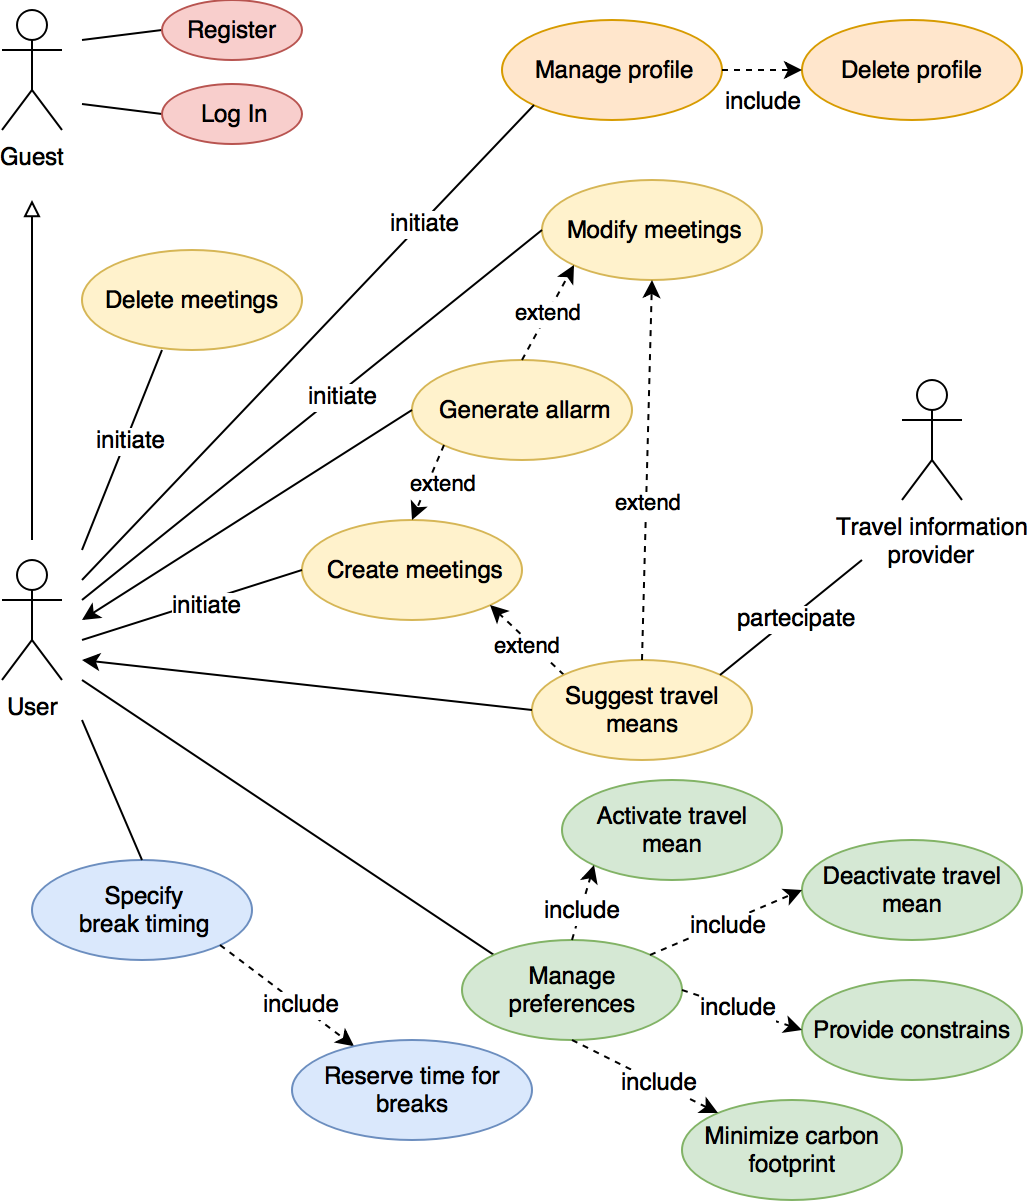
\includegraphics[width=0.75\textwidth]{img/diagrams/uc.png} \\ \bigskip
		Figure 2.1: Use Case Model. Explains actors and functionalities offered by the system.
		\label{default}
		\end{center}
	\end{figure}
	
	
	\subsection{User Characteristics}
	The target user is someone who needs an automated system to manage appointments and schedules the travels.

	The meeting should not overlap with any pre - existing one and the app should allow the user to move from his/her present position to the meeting site, using the means of transport preferred and according to traffic conditions. 
	
	
	\subsection{Assumptions and Dependences}
	The following assumptions are given for granted:
	\begin{itemize}
		\item  Transport means comply with user’s requests.
		\item  The device is always connected to the server.
		\item  All users provide correct and valid data at time of registration.
		\item  GPS shows the actual position of the owner.
		\item  The system can rely on a \textit{Travel information provider} that gives correct and updated information about travel means paths and timetables.
		\item  The event, when inserted, modified or deleted, must not be in the past.
	\end{itemize}
	
	
	\subsection{Constraints}
	
	
	\subsubsection{Regulatory policies}
	The application must be allowed by the user to collect his/her position, through GPS.
	
	
	\subsubsection{Hardware limitations}\label{ref1}
	\begin{itemize}
		\item Web application:
			\begin{itemize}
				\item Internet connection;
				\item 800x600 screen resolution;
				\item JavaScript enabled.
			\end{itemize}
		\item Mobile application:
			\begin{itemize}
				\item Internet connection;
				\item 50 MB of available storage space;
				\item 1GB of RAM;
				\item GPS module.
			\end{itemize}
	\end{itemize}
	
	
	\subsubsection{Reliability requirements}
	The system reliability, that is the probability to operate without a failure for a specific period of time, must be at least 99\%.
	
	
	\subsection{World and Machine model interpretation}
	In this part of RASD, a description of the system-to-be is provided following the World and Machine model introduced by Jackson and Zave.
	
	\bigskip
	They indicate as the Machine the portion of the system-to-be developed, typically software-to-be plus hardware. The Machine domain is the set of phenomena located entirely in the machine and that the machine control (e.g., machine algorithms, controlled device, ...)
	
	\bigskip
	Opposite, the World domain is a set of phenomena that the machine cannot observe.

	\bigskip
	The World is connected with the Machine through Shared Phenomena part of it both observed by the Machine and by the World themselves. The Shared Phenomena can be controlled by the World and observed by the Machine or controlled by the Machine and observed by the World.
	
	\bigskip
	\bigskip
	\begin{center}
		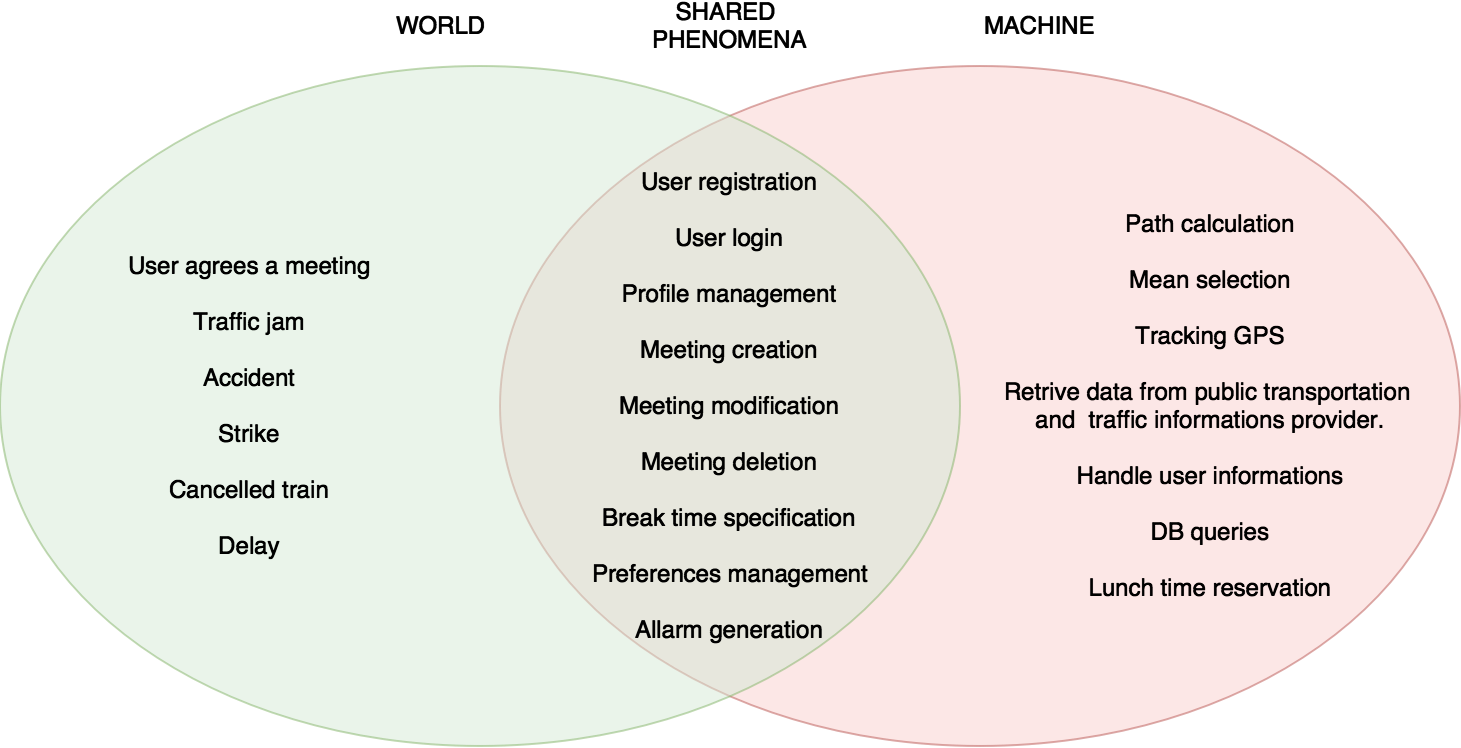
\includegraphics[width=\textwidth]{img/diagrams/world_machine.png} \\ \bigskip
		Figure 2.2: World and Machine model for the main functionalities offered by the system.
	\end{center}
	
	\section{Specific Requirements}
	
	
	\subsection{External Interface Reqirements}
	
	
	\subsubsection{User Interfaces}
	The user interface must be intuitive and unified, granting to the user a pleasant experience. In order to make it possible both web and mobile application must satisfy the following requirements:
	\begin{itemize}
		\item If the session is not already active the user must be redirected to a Login page. If he/she is not already registered he/she can create a new account within the same page. Moreover, the user must be able to Sign In/Sign Up not only with username and password but also with his/her social accounts (e.g. Google, Facebook, Twitter);
		\item Once logged, the user must be redirected to his/her personal page;
		\item A toolbar must allow the user to navigate through the pages described below;
		\item The user's personal page must display an overview of user's future events (display them in a list, in a calendar or in a map) and must also offer the possibility to insert new ones;
		\item Clicking on an event the user must be redirected to the event's detail page;
		\item The event's detail page must display detailed information such as location of the event, time and suggested mean (including the path)  needed to reach it;
		\item The event's detail page must allow the user to modify or delete the event;
		\item If an user tries to insert or modified an event which location is unreachable in the remaining time an alert should be displayed;
		\item The Account settings page must allow the user to modify its/her personal informations or delete the account;
		\item The user must be allowed to select between different languages (en, it, de, fr, es, ru, zh, ja, ar);
		\item The UI must comply the Flat Design principles;
		\item Both web and mobile applications must use the same graphic objects for the same interface elements.
	\end{itemize}
	
	\bigskip
	\bigskip
	Specific constraints must be satisfied by specific application:
	\begin{itemize}
		\item Web application:
			\begin{itemize}
				\item The user interface must be responsive i.e. adapt to screen size;
				\item All pages must comply W3C standards.
			\end{itemize}
		\item Mobile application:
			\begin{itemize}
				\item Must run on iOS 9.3 or greater and Android 5.0 or greater.
			\end{itemize}
	\end{itemize}

	
	
	\subsubsection{Hardware Interfaces}
	As already mentioned in section 2.1.2, the web application can be executed on any computer that meets the basic requirements described in the "Hardware Limitation" section.
	
	\bigskip
	The mobile application must exchange data with the GPS module located on any type of smartphone or tablet. You must also have an internet connection to communicate with the main system server.

	
	\subsubsection{Software Interfaces}
	The backend application requires the following software products:
	\begin{itemize}
		\item Java EE 7 - http://www.oracle.com/technetwork/java/javaee/overview/index.html
		\item MySQL 5.7 - http://dev.mysql.com/
	\end{itemize}
	
	\bigskip
	As mentioned in Section 2.1.3, the backend must interfaced with the APIs of a public transportation and  traffic informations provider, to have the information useful to plan the path.
	
	\bigskip
	The mobile applications requires the following software products:
	\begin{itemize}
		\item (iOS) Swift 4 - https://developer.apple.com/swift/
		\item (Android) Java SE 7 - http://www.oracle.com/technetwork/java/javase/overview/index.html
	\end{itemize}

	
	\subsubsection{Communications Interfaces}
	Every communication between application server and client must comply the HTTPS protocol.
	
	\bigskip
	If the back-end application and the DBMS runs on different servers the communication between them must be SSL/TLS encrypted.
	
	
	\subsection{Functional requirements}
	
	
	\subsubsection{Register}
	
	\bigskip
	\noindent
	\textbf{Purpose} \\
	Anyone who want to subscribe to Travlendar + can make the registration process through the mobile app or the web site.
	The guest must first complete the registration form with personal data (i.e., first name, last name, birth, sex, e-mail, password) and accept terms on data protection and conditions.
	
	Once the information are submitted, the system checks them and sends a confirmation email. If the operation is successful, the guest becomes a user and may start using the application.

	\bigskip
	\noindent
	\textbf{Scenario 1} \\
	Allyson wants to register Travlendar + using the web page. She opens the home page of a search engine and types "travlendar +". When you reach home page of Travlendar, click on “Sign up” and the registration form appears. She types in her data, such as first name, last name, birthdate, sex, email and password, and accepts the terms of data protection. At the end she clicks on the "Done" button, and after a few seconds she will receives an email confirming her registration.

	\bigskip
	\noindent
	\textbf{Scenario 2} \\
	Benjamin has just moved to London and his friend Carl has spoken to him about  Travlendar +, so he decides to sign up in order to manage better his new meetings. He downloads the app on his mobile phone and opens it. The home page appears and he clicks on "Sign up". The registration form appears. He inserts types in his personal data and clicks on “Done”. Immediately after his click, a message informs him that his password has been already used.
	
	\newpage
	\noindent
	\textbf{Use cases} \\

	\begin{center}
		Table 3.1: Register use case.
		
		\bigskip
		\begin{tabular}{p{0.3\textwidth}|p{0.6\textwidth}}
	   		\hline
	    		Actor & Guest \\ \hline
	    		Goal & Goal 1 \\ \hline
	    		Input Condition & The person wants to subscribe to the service \\ \hline
	    		Event flow & 
			\begin{enumerate}
	  			\item The guest opens the home page or mobile application of "Travlendar +"  and clicks the "Sign up" button;
	  			\item The registration form appears and the guest completes the mandatory fields;
	  			\item The guest allows the personal data processing to be marked on the corresponding box;
	  			\item The guest clicks on "Done" button;
	  			\item The system saves the information in the database and sends an email to the guest confirming his/her subscription and that he/she has become a user of the service.
	 		 \end{enumerate} \\ \hline
	    		Output Condition & The system informs the user that he/she has registred successfully. \\ \hline
	    		Exception & The system can report alert messages when a non valid or already used mail address is typed in. Another exception can be reported if the license number does not exist or when the terms and conditions of use are not accepted. \\ \hline
	    	\end{tabular}
	\end{center}
	
	\bigskip
	\noindent
	\textbf{Functional requirements} \\
	
	\begin{itemize}
		\item The system must not accept an email address already used during the registration procedure.
		\item The system requires the following mandatory personal information:
			\begin{itemize}
				\item First name
				\item Last name
				\item Sex
				\item Date of birth
				\item Address
				\item E-mail address
				\item Password
				\item Driving license number (optional)
			\end{itemize}
		\item If the terms and conditions of use and data protection are not accepted, the system must not complete the registration procedure.
		\item As soon as the guest clicks on "Done", the system sends automatically an email of confirmation.
		\item The guest can leave the registration procedure at any time.
	\end{itemize}

	\newpage
	\noindent
	\textbf{Activity diagram} \\

	\begin{figure}[h!]
		\bigskip
		\centering
		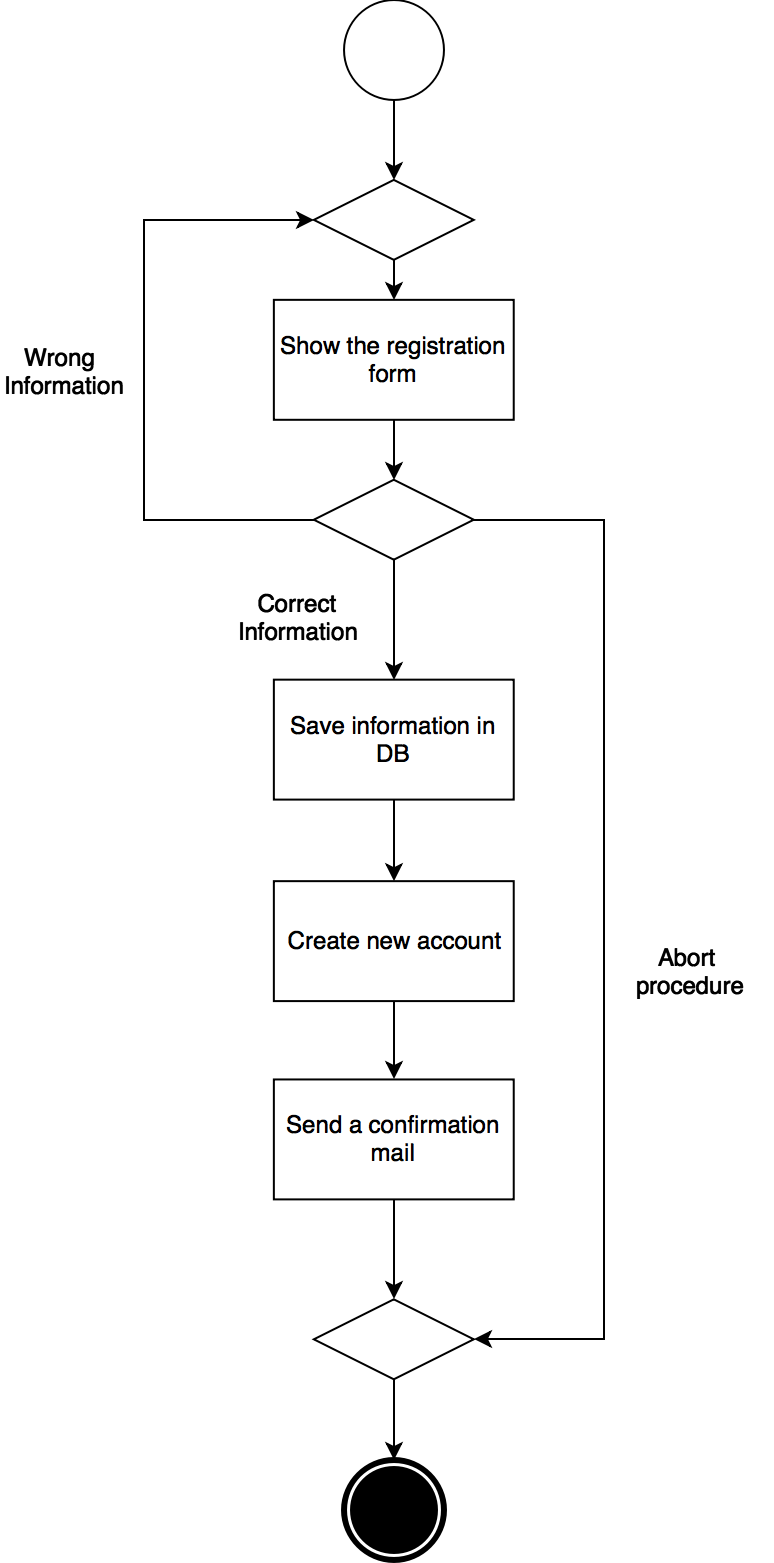
\includegraphics[scale=0.22]{img/diagrams/register_ad.png}
		\caption{Activity diagram for Register.}
	\end{figure}

	\begin{figure}[h!]
		\bigskip
		\centering
		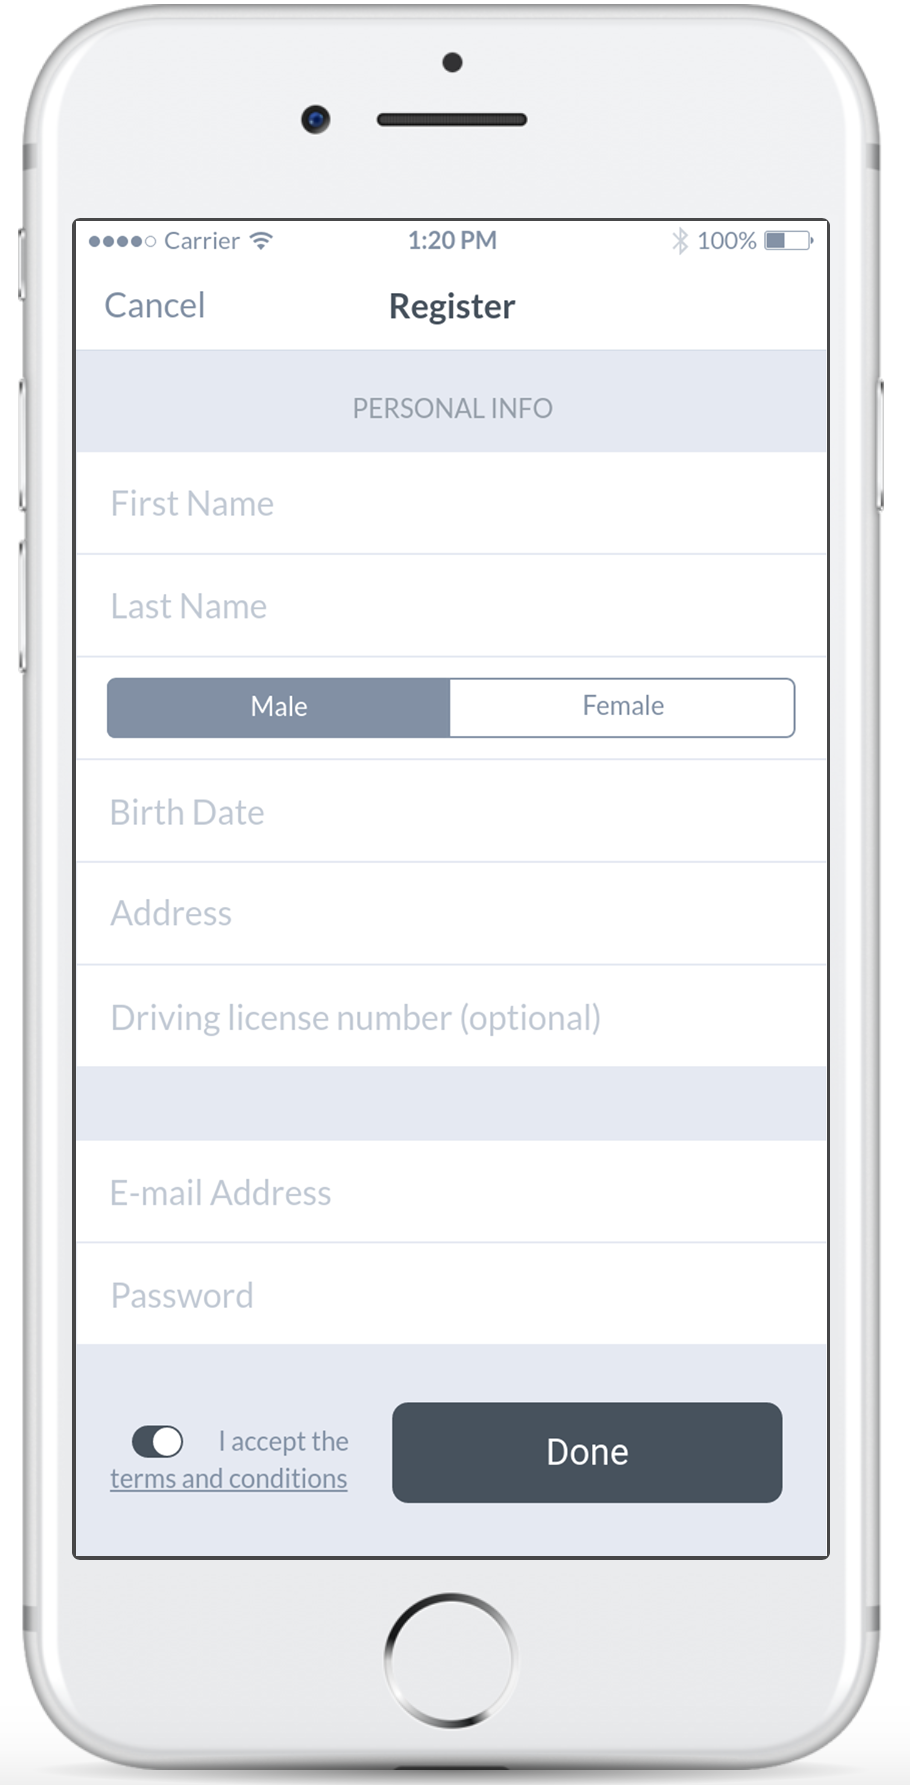
\includegraphics[scale=0.20]{img/mockups/mobile/register.png}
		\caption{Mockup for registration on a mobile device.}
	\end{figure}

	\newpage
	\subsubsection{Login}
	
	\bigskip
	\noindent
	\textbf{Purpose} \\
	The Login phase aims to guarantee the access to authorized users. Access can be made by inserting mail and password, or via a social network account (i.e., \textit{Facebook}, \textit{Instagram}, \textit{Linkedin}).
	
	If the user forgets his/her password, it is also possible to retrieve it clicking on "Forgot Password?". Once the button is clicked, an email with credentials is sent.


	\bigskip
	\noindent
	\textbf{Scenario 1} \\
	Catherine wants to enter a new meeting in her calendar. She accesses the "Travlendar +" home page on her laptop entering her personal email and password (registered when she signed up). She clicks then on "Sign in" and gets in as authorized user because everything is correct.
	
	\bigskip
	\noindent
	\textbf{Scenario 2} \\
	Dominique wants to insert his check up to the dentist on next Tuesday. He opens the app on his mobile phone and types his credentials. However there is a problem now: he can't remember the password used when authenticated himself. Dominique clicks therefore on "Forgot password?" button. The system forwards to the email address recorded a new password.
	
	\bigskip
	\noindent
	\textbf{Use cases} \\
	
	\begin{center}
		Table 3.2: Login use case.
		
		\bigskip
    		\begin{tabular}{p{0.3\textwidth}|p{0.6\textwidth}}
   			\hline
    			Actor & User \\ \hline
    			Goal & Goal 1 \\ \hline
    			Input Condition & A user already registered, wants to login. \\ \hline
    			Event flow & 
			\begin{enumerate}
  				\item The user opens the home page or the mobile application and the system shows the login page;
  				\item The user inserts his/her email address and password;
  				\item The user clicks on "Sign in" button.
 			\end{enumerate} \\ \hline
    			Output Condition & The system connects the user to his / her personal page. \\ \hline
    			Exception & The exception that may arise is the inputting of an insertion mail or an incorrect password. The system sends the user an error message asking him/her to verify the address and/or the password re-enter them. \\ \hline
    		\end{tabular}
	\end{center}
	
	\bigskip
	\noindent
	\textbf{Functional requirements} \\
	\begin{itemize}
		\item The user must have been already registered with the system for successful login.
		\item The user must have correct email and password available to successfully login.
		\item The user must use a password connected to a specific email address.
		\item Bad credentials must not allow the user authentication.
		\item If the user clicks on "Forgot password?" the system must send a link where the user can reset his/her password.
		\item When a new password has been set, the system must allow the user to authenticate only with new credentials.
	\end{itemize}
	
	\newpage
	\noindent
	\textbf{Activity diagram} \\
	
	\begin{figure}[h!]
		\bigskip
		\centering
		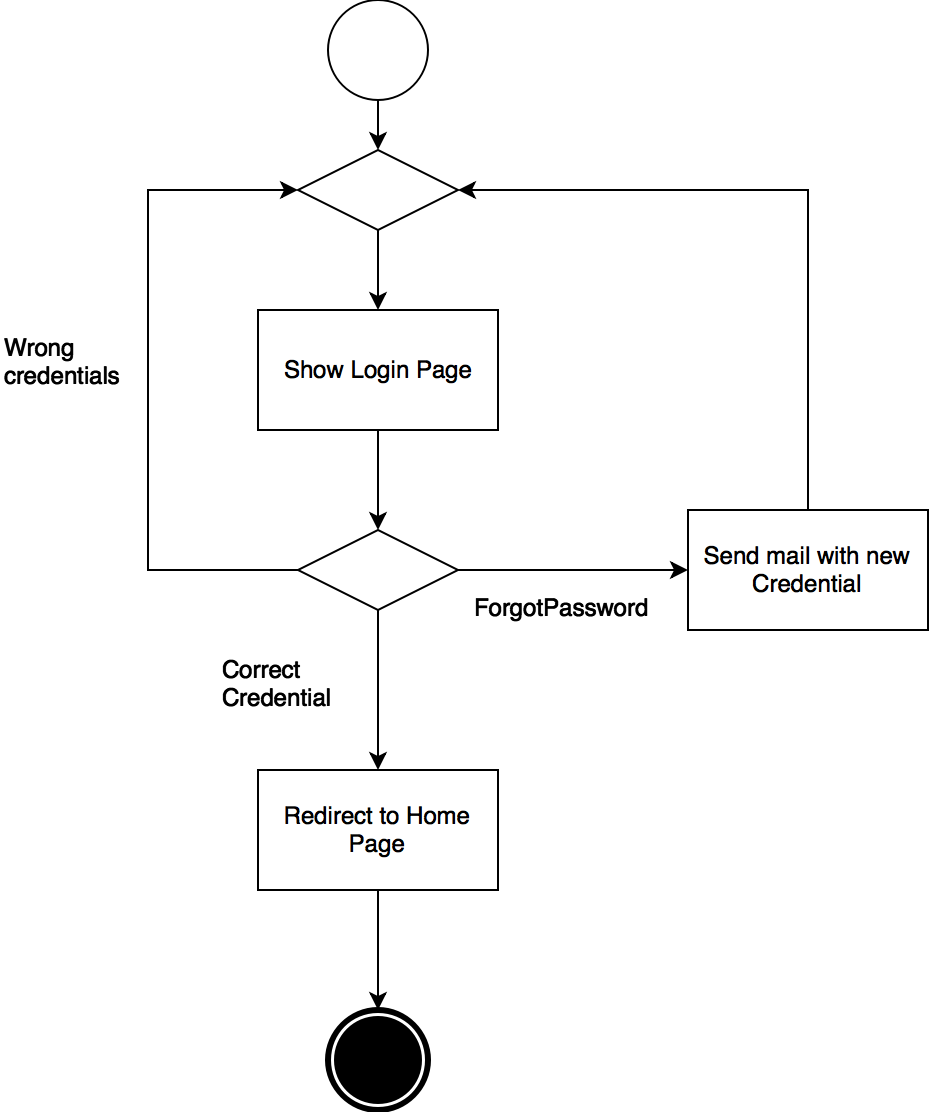
\includegraphics[scale=0.25]{img/diagrams/login_ad.png}
		\caption{Activity diagram for Login.}
	\end{figure}
	\begin{figure}[h!]
		\bigskip
		\centering
		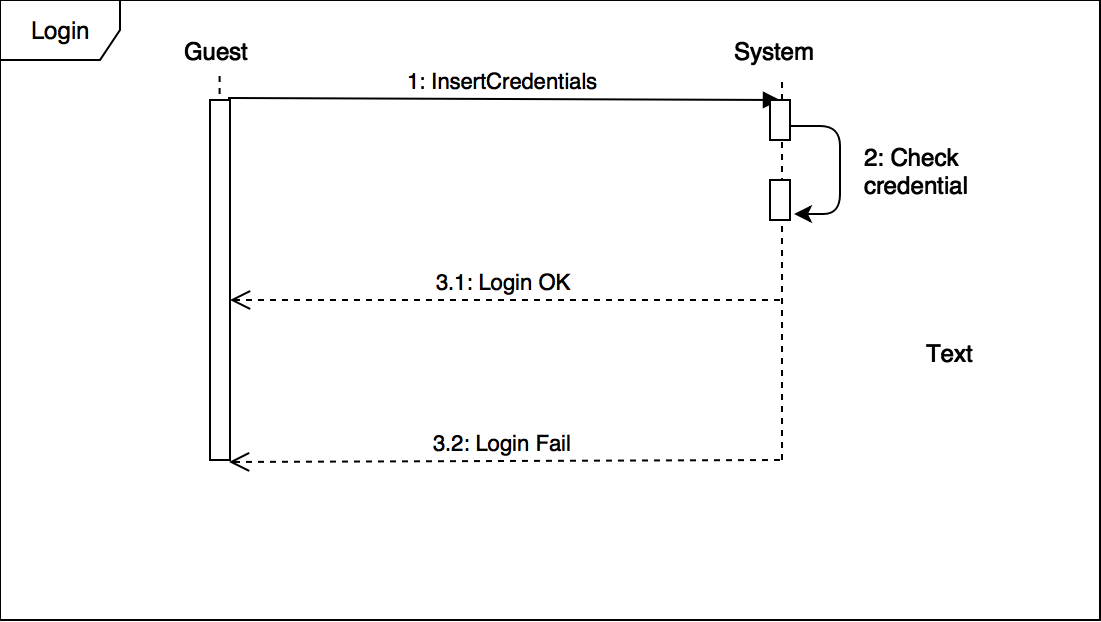
\includegraphics[scale=0.25]{img/diagrams/login_sd.png}
		\caption{Login sequence diagram.}
	\end{figure}
	\begin{figure}[h!]
		\bigskip
		\centering
		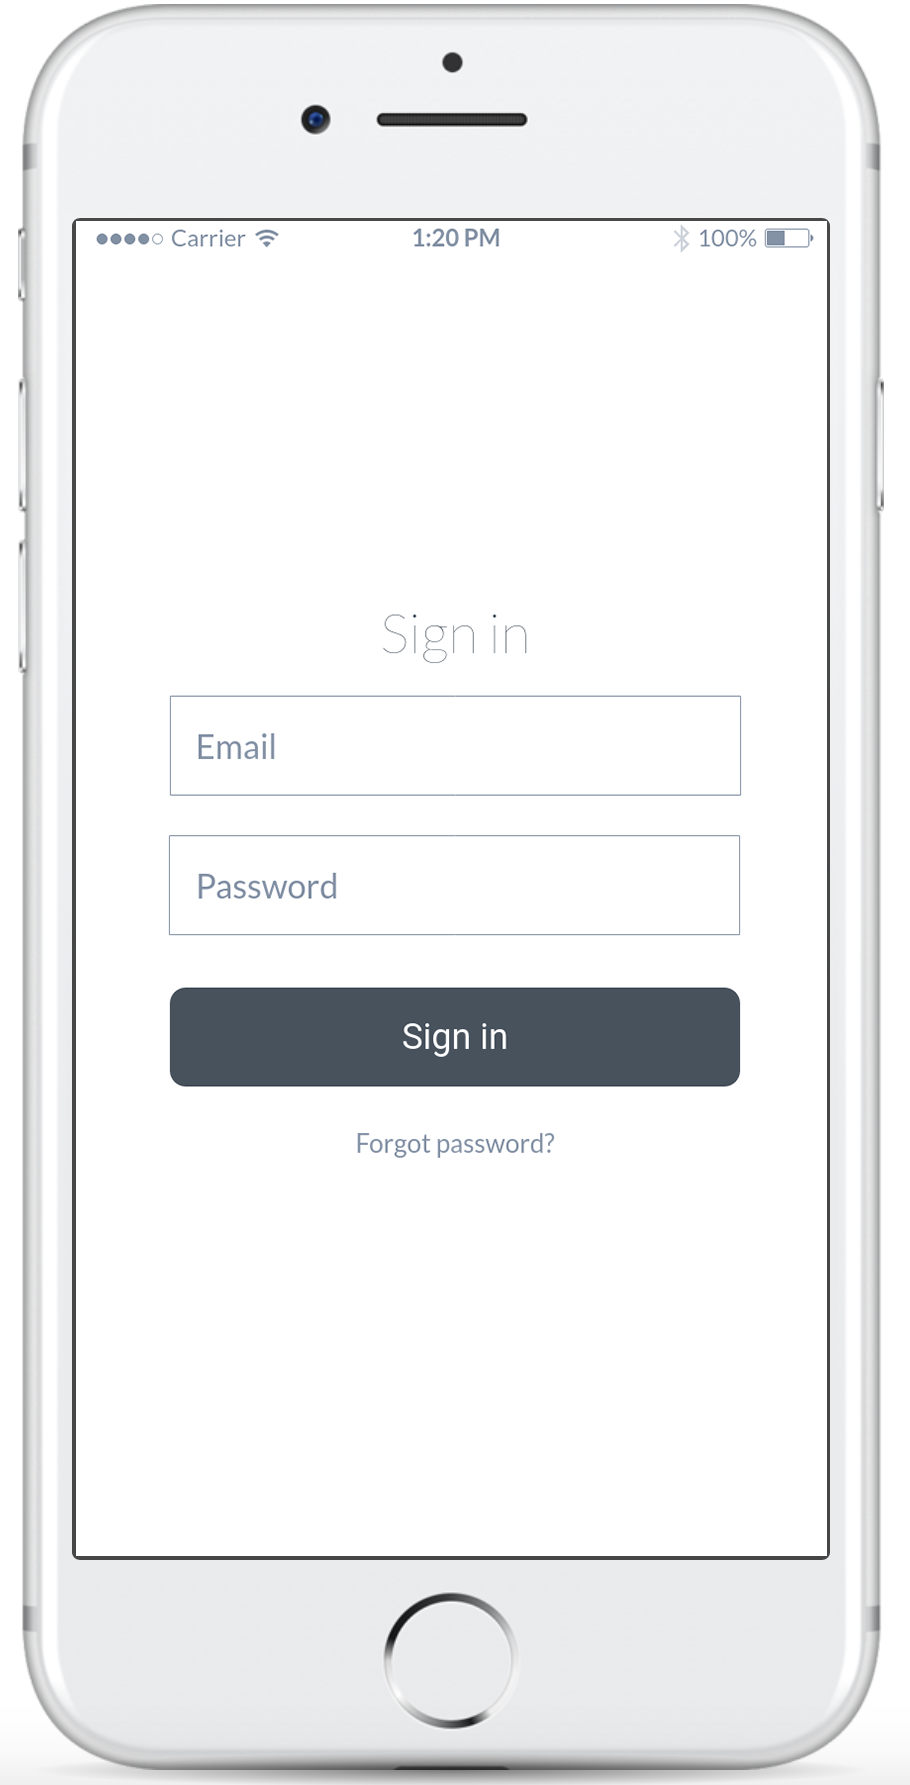
\includegraphics[scale=0.25]{img/mockups/mobile/login.png}
		\caption{Mockup for Login on a mobile device.}
	\end{figure}
	
	\newpage
	\subsubsection{Create meetings}
	
	\bigskip
	\noindent
	\textbf{Purpose} \\
	The purpose is to allow the authorized user to create a new meeting on the calendar by entering the meeting name, date, time, place, and also specifying how to reach the site. The task of the system is to check this information and, if incorrect, alert the user to modify them.
	
	\bigskip
	\noindent
	\textbf{Scenario 1} \\
	Emma has to enter a driving lesson for tomorrow. Then she logs in her "Travlendar +" personal page as authorized user and press the "New event" button to create the appointment. Then the system open a form where she must enter the name of the event, date, time and place. Once completed, she press "Save" button. The system verifies the correctness of the information, calculates the most appropriate way to reach it and creates the event on the calendar.
	
	\bigskip
	\noindent
	\textbf{Scenario 2} \\
	Franklin just took an appointment from the hairdresser in half an hour. He has decided afterward to create an appointment on her mobile app "Travelendar +". Log in with your smartphone and press the "+" button. A form appears to be completed with the event, date, time and place. Once the form is completed, submit it. The system checks the information and issues an error message because the site can not be reached in half an hour by bike (Franklin’s only active travel mean is bike sharing service).
	
	\bigskip
	\noindent
	\textbf{Use cases} \\
	
	\begin{center}
		Table 3.3: Create meetings use case table.
		
		\bigskip
    		\begin{tabular}{p{0.3\textwidth}|p{0.6\textwidth}}
   		 	\hline
    			Actor & User \\ \hline
    			Goal & Goal 4 \\ \hline
    			Input Condition & An user wants to create a new meeting on his/her calendar.\\ \hline
    			Event flow & 
			\begin{enumerate}
  				\item The user must login by entering his/her mail and password;
  				\item The user clicks the "+" / "New event" button to create a new meeting;
  				\item The system shows the form to be filled;
  				\item The user fulfills the form and clicks on "Save";
  				\item The system checks the information, calculates the most appropriate way to reach the meeting's location and saves them in the database; in the case of incorrect information, the user alerts you with an error message.
 			 \end{enumerate} \\ \hline
    			Output Condition & The system creates a new meeting on the user's calendar in the home page. \\ \hline
    			Exception & The exception might be generated when the mean to reach the site is not valid (e.g., if you have to drive on a motorway, you cannot use the bicycle), or your downtime is less than the time you need. Another exception is raised if the date creating the meeting is later than the date of the meeting. \\ \hline
    		\end{tabular}
	\end{center}
	
	\bigskip
	\begin{figure}[h!]
		\bigskip
		\centering
		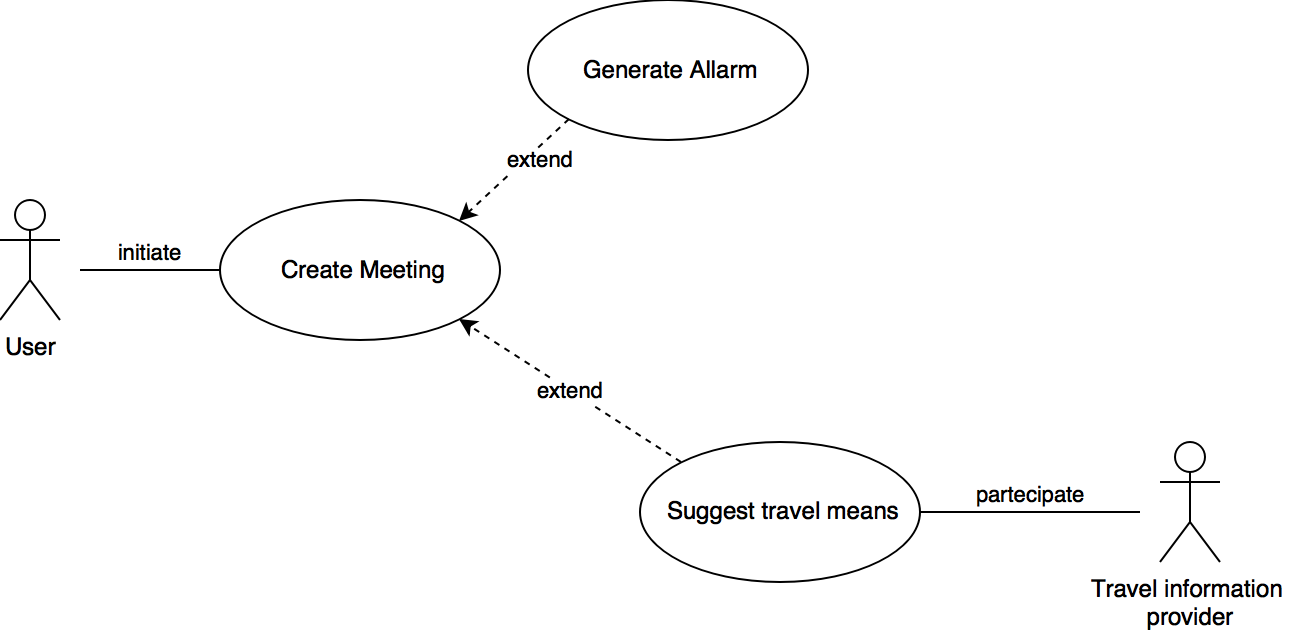
\includegraphics[scale=0.25]{img/diagrams/create_meeting_uc.png}
		\caption{Create meeting Use case diagram.}
	\end{figure}
	
	\bigskip
	\noindent
	\newpage
	\textbf{Functional requirements} \\
	\begin{itemize}
		\item The user must log in successfully;
		\item The user must insert the following information in the form:
			\begin{itemize}
				\item Name
				\item Start time
				\item End time
				\item Meeting location
				\item People number
			\end{itemize}
		\item The system must verify that the meeting's date is later than the creation date;
		\item The system must check that the way to reach is compatible with the path;
		\item The system must verify that the time available is sufficient to reach the appointment site;
		\item After verification of the correctness of the information, the system must create the meeting on the personal calendar;
		\item The system must send an error message in case of inappropriate data or mean.
	\end{itemize}
	
	\newpage
	\noindent
	\textbf{Activity diagram} \\
	
	\begin{figure}[h!]
		\bigskip
		\centering
		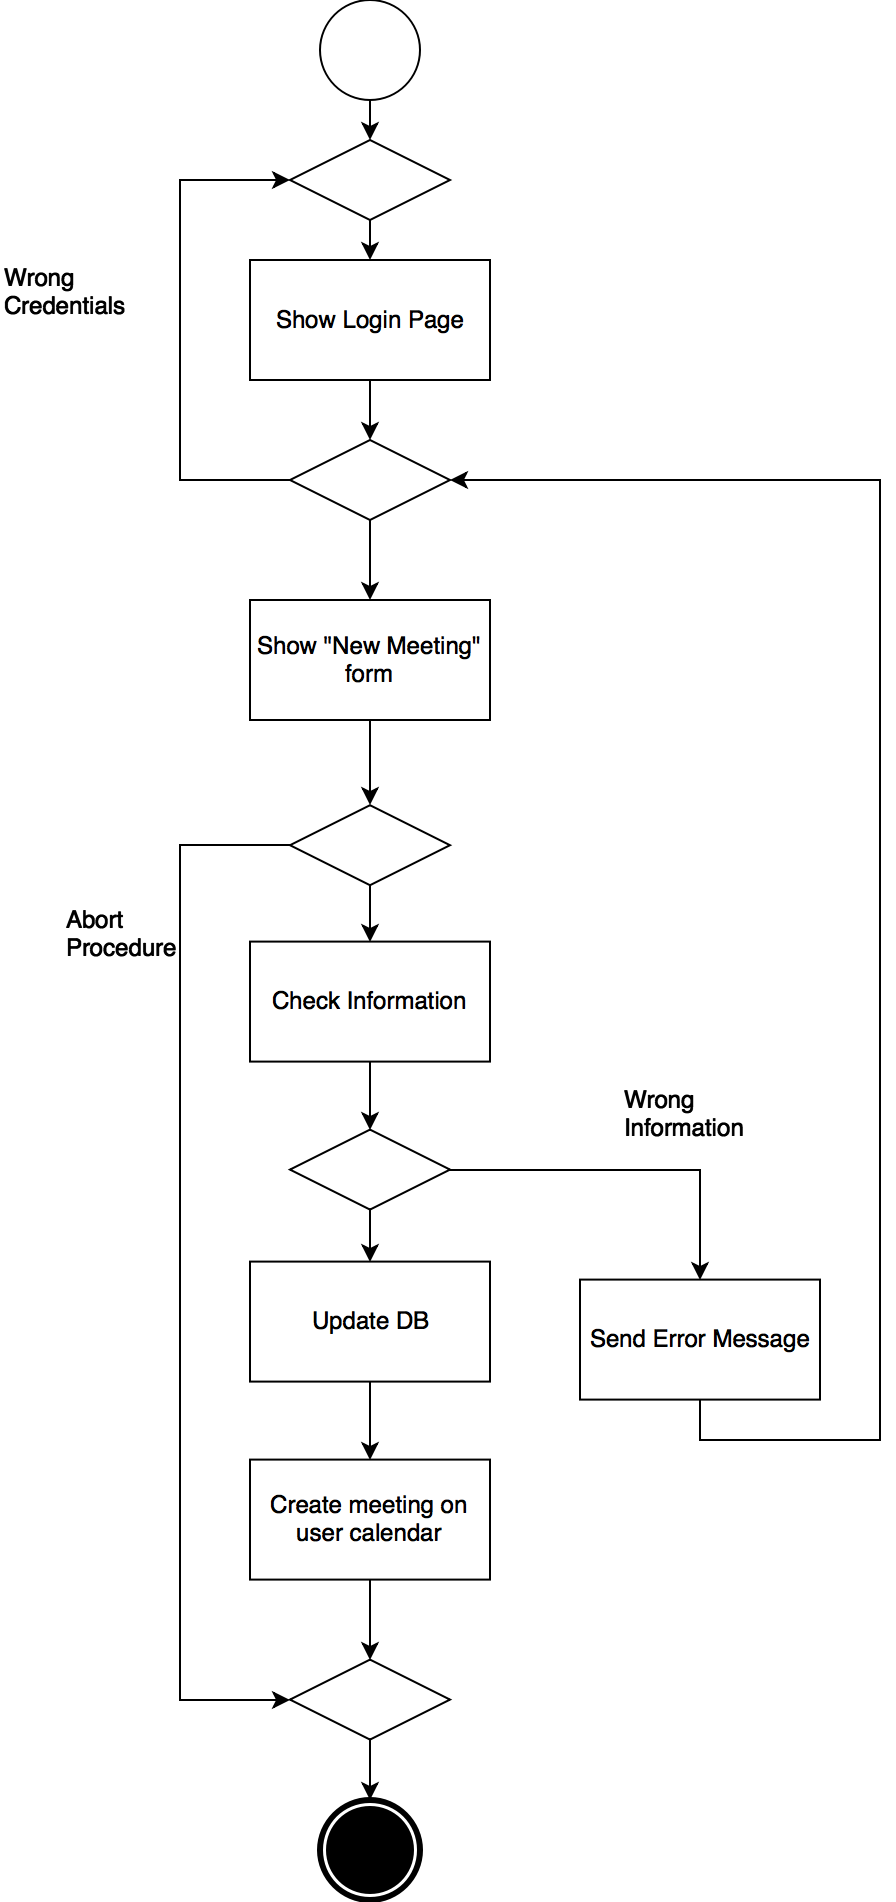
\includegraphics[scale=0.25]{img/diagrams/create_meetings_ad.png}
		\caption{Activity diagram for Create meetings.}
	\end{figure}
	

	\subsubsection{Modify meetings}
	
	\bigskip
	\noindent
	\textbf{Purpose} \\
	The purpose of this part is to allow the user, after saving a meeting on the calendar, to be able to modify some information (such as date, time, number of people, place, means of transport). The system must verify the compatibility of the modification.
	
	\bigskip
	\noindent
	\textbf{Scenario 1} \\
	Gordon was just called by the school secretary and was advised that he had a lesson in IIIA class at 10 a.m. instead of at 9 a.m. on Thursday. Enter the personal page of "Travlendar +" and select the appointment. Press the "Modify" button next to the selected event. The system shows the form already completed and Gordon changes the time. Press  "Save" button. The system checks the information and updates successfully the appointment.
	
	\bigskip
	\noindent
	\textbf{Scenario 2} \\
	Helen has to hold a conference in Paris. Now she is at Milan Malpensa Airport and she has just been notified that the plane has 120 minutes delay. He decides to change the meeting to control if she can reach the conference place in time. Enter your personal page through the mobile application. Helen selects the meeting and presses the "Modify" button. Then, she changes the times in the form and presses "Save". The system verifies the information and sends an error message because changing the time the plane can't  reach Paris in time for the conference.
	
	\bigskip
	\noindent
	\textbf{Use cases} \\
	
	\begin{center}
		Table 3.4: Modify meetings use case.
		
		\bigskip
    		\begin{tabular}{p{0.3\textwidth}|p{0.6\textwidth}}
   			\hline
    			Actor & User \\ \hline
    			Goal &  Goal 5 \\ \hline
    			Input Condition & The user wants to modify a meeting on his/her calendar. \\ \hline
			Event flow & 
			\begin{enumerate}
  				\item The user must login entering his/her email and password;
  				\item The user selects the meeting he/she wants to modify with one click;
  				\item The system shows a dialog box with "Modify" and "Delete" buttons;
  				\item The user presses the "Modify" button;
  				\item The system shows the form with the meeting information;
  				\item The user modifies the form and presses the "Save" button;
  				\item The system verifies the information and saves it in the database; in the case of incorrect information, the system alerts the user with an error message.
 			 \end{enumerate} \\ \hline
    			Output Condition & The system modifies a meeting on the calendar on the user's home. \\ \hline
    			Exception & The exceptions that can be raised are the same as those for creating the event. The exception that may be raised is that the way to reach the site is not valid (for example, if you have to drive a motorway, you can not use the bicycle), or your downtime is less than the time you need. Another exception is raised if the meeting change date is later than the date of the meeting. \\ \hline
    		\end{tabular}
	\end{center}
	
	\newpage
	\noindent
	\textbf{Functional requirements} \\
	\begin{itemize}
		\item The user must log in successfully;
		\item The user must have already created an event;
		\item The user must change one or more of the following information in the form:
			\begin{itemize}
				\item Name
				\item Start time
				\item End time
				\item Meeting location
				\item People number
			\end{itemize}
		\item The system must verify that the date of the event is after the creation date;
		\item The system must check that the way to reach is compatible with the path;
		\item The system must verify that the time range is sufficient to reach the appointment place;
		\item Once the information is verified, the system has to change the appointment on the personal calendar;
		\item The system must send an error message in case of inappropriate date or time.
	\end{itemize}
	
	\newpage
	\noindent
	\textbf{Activity diagram} \\
	
	\begin{figure}[h!]
		\bigskip
		\centering
		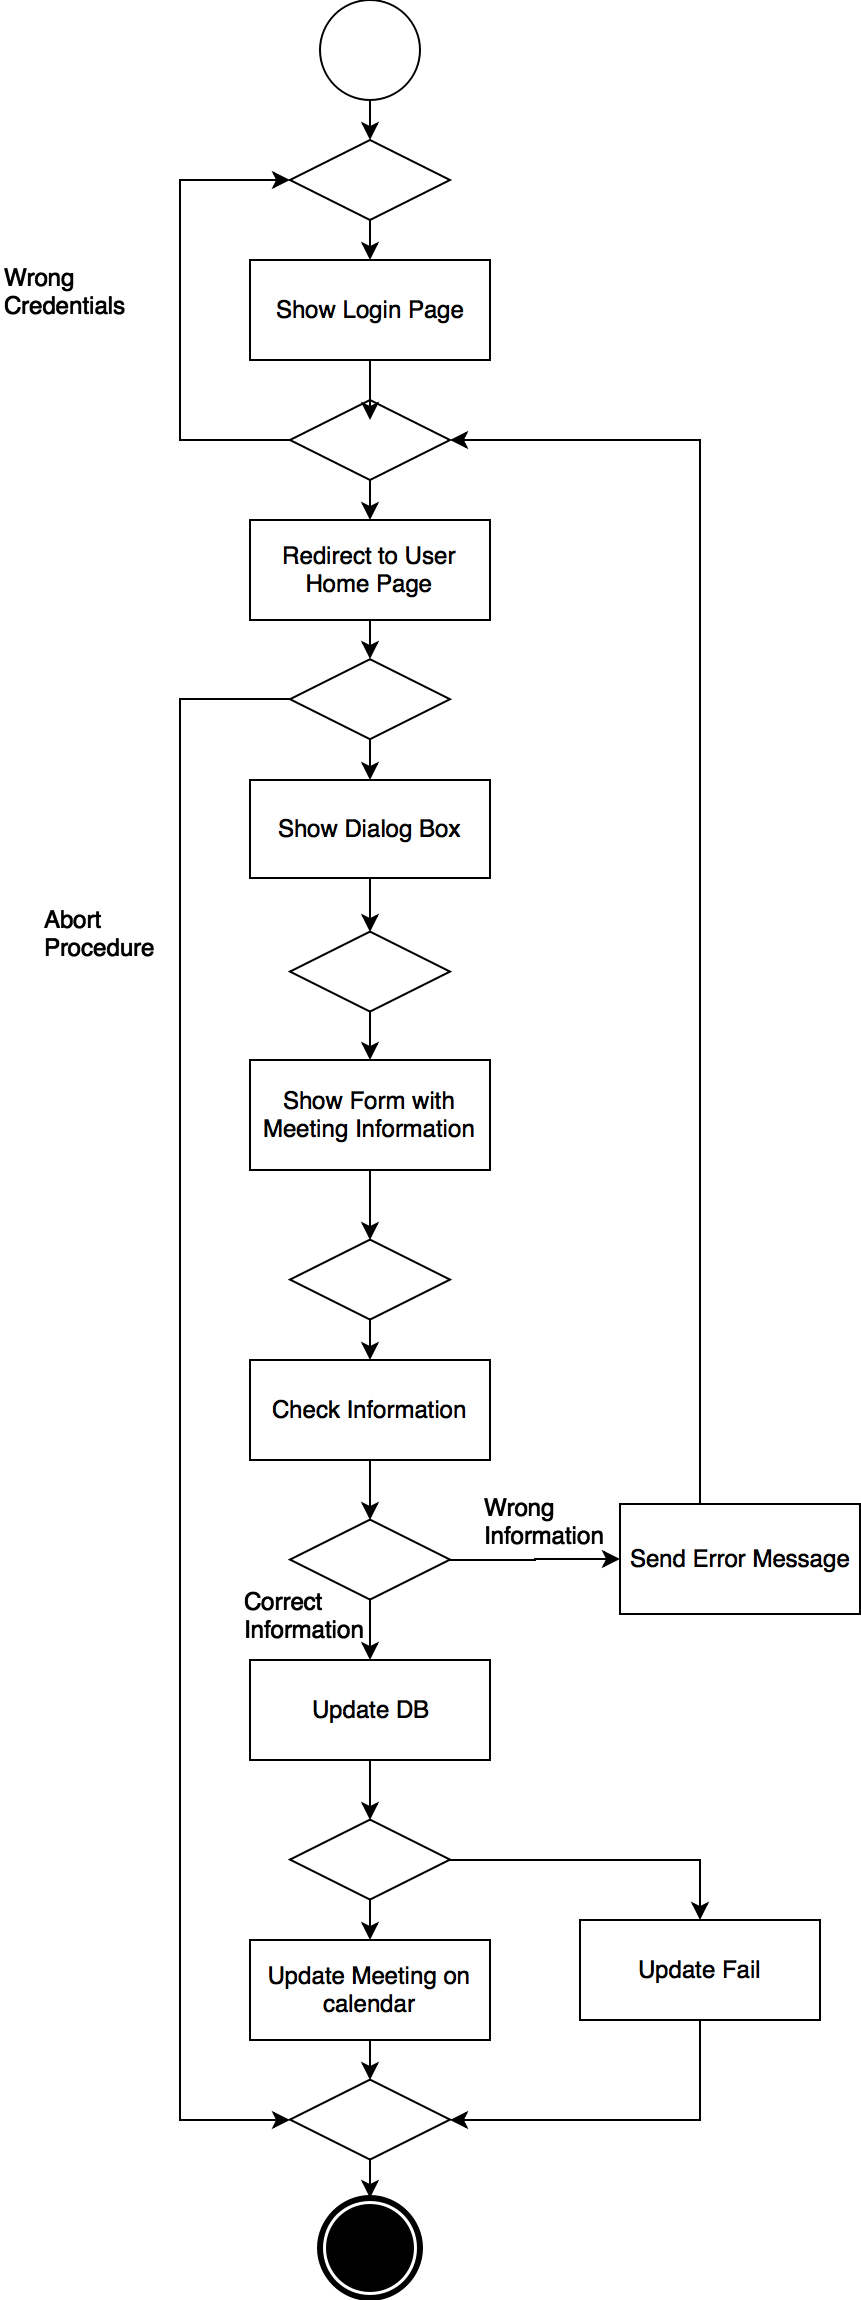
\includegraphics[scale=0.25]{img/diagrams/modify_meetings_ad.png}
		\caption{Activity diagram for Modify meetings.}
	\end{figure}

	\begin{figure}
		\centering
		\begin{minipage}{.45\textwidth}
			\centering
			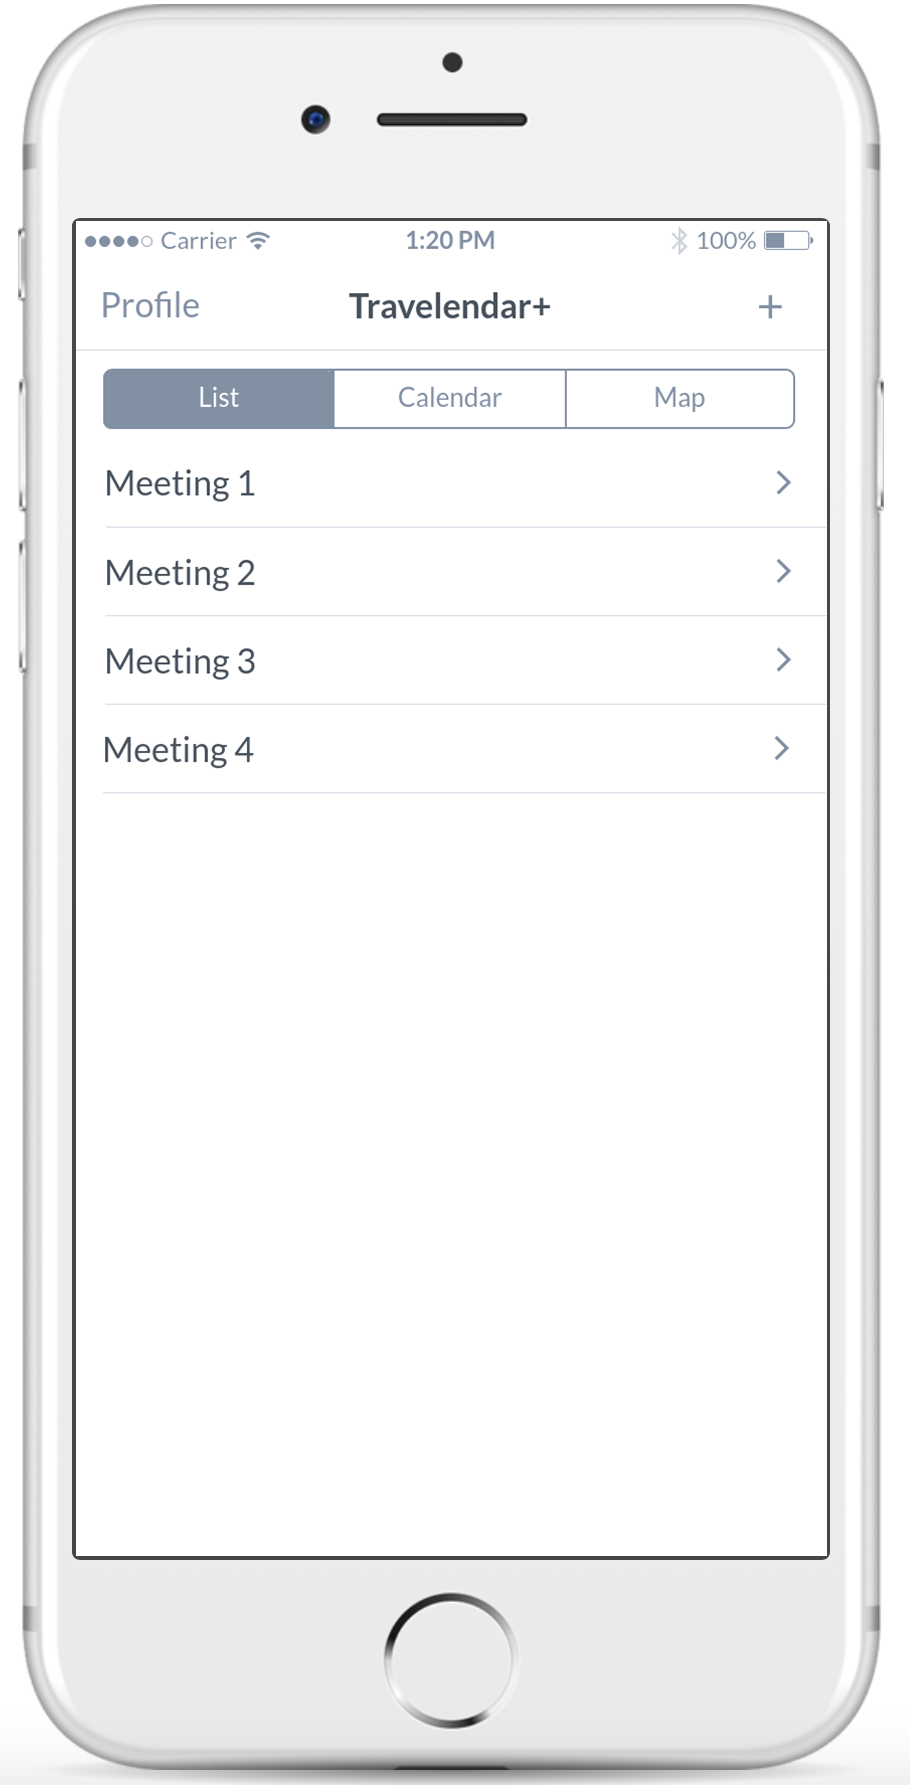
\includegraphics[width=.4\linewidth]{img/mockups/mobile/list.png}
			\caption{Meetings list view on mobile.}
			\label{fig:test1}
		\end{minipage}
		\begin{minipage}{.45\textwidth}
			\centering
			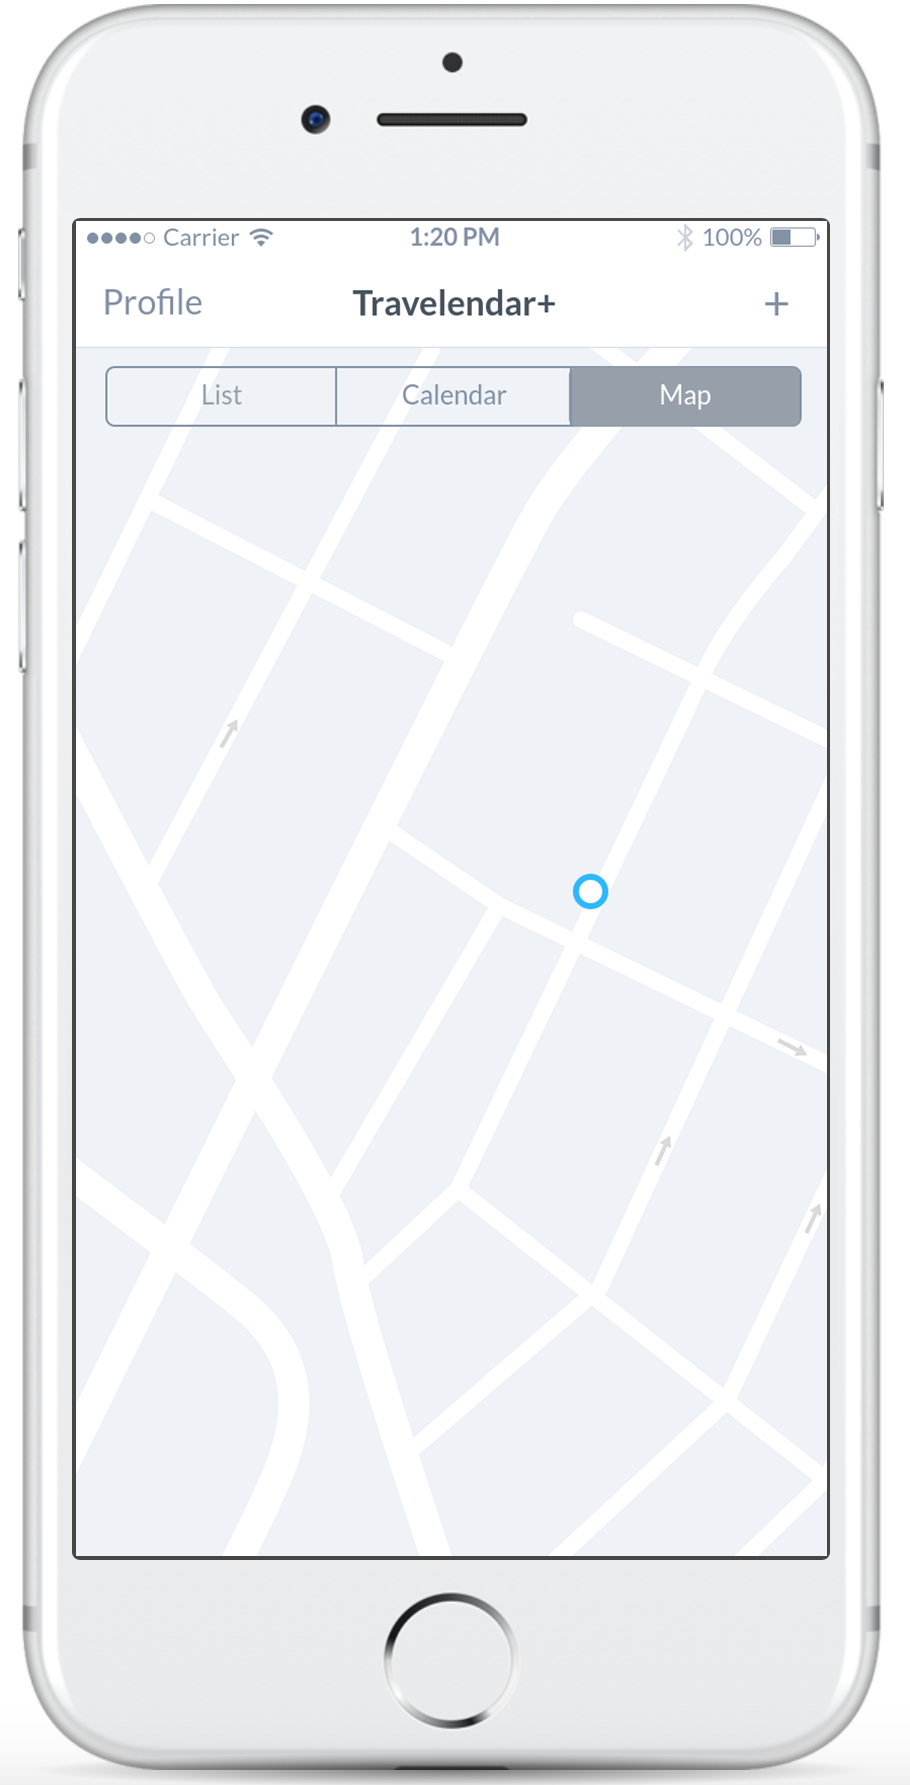
\includegraphics[width=.4\linewidth]{img/mockups/mobile/map.png}
			\caption{Meetings map view on mobile.}
			\label{fig:test2}
		\end{minipage}
	\end{figure}
	\begin{figure}[h!]
		\bigskip
		\centering
		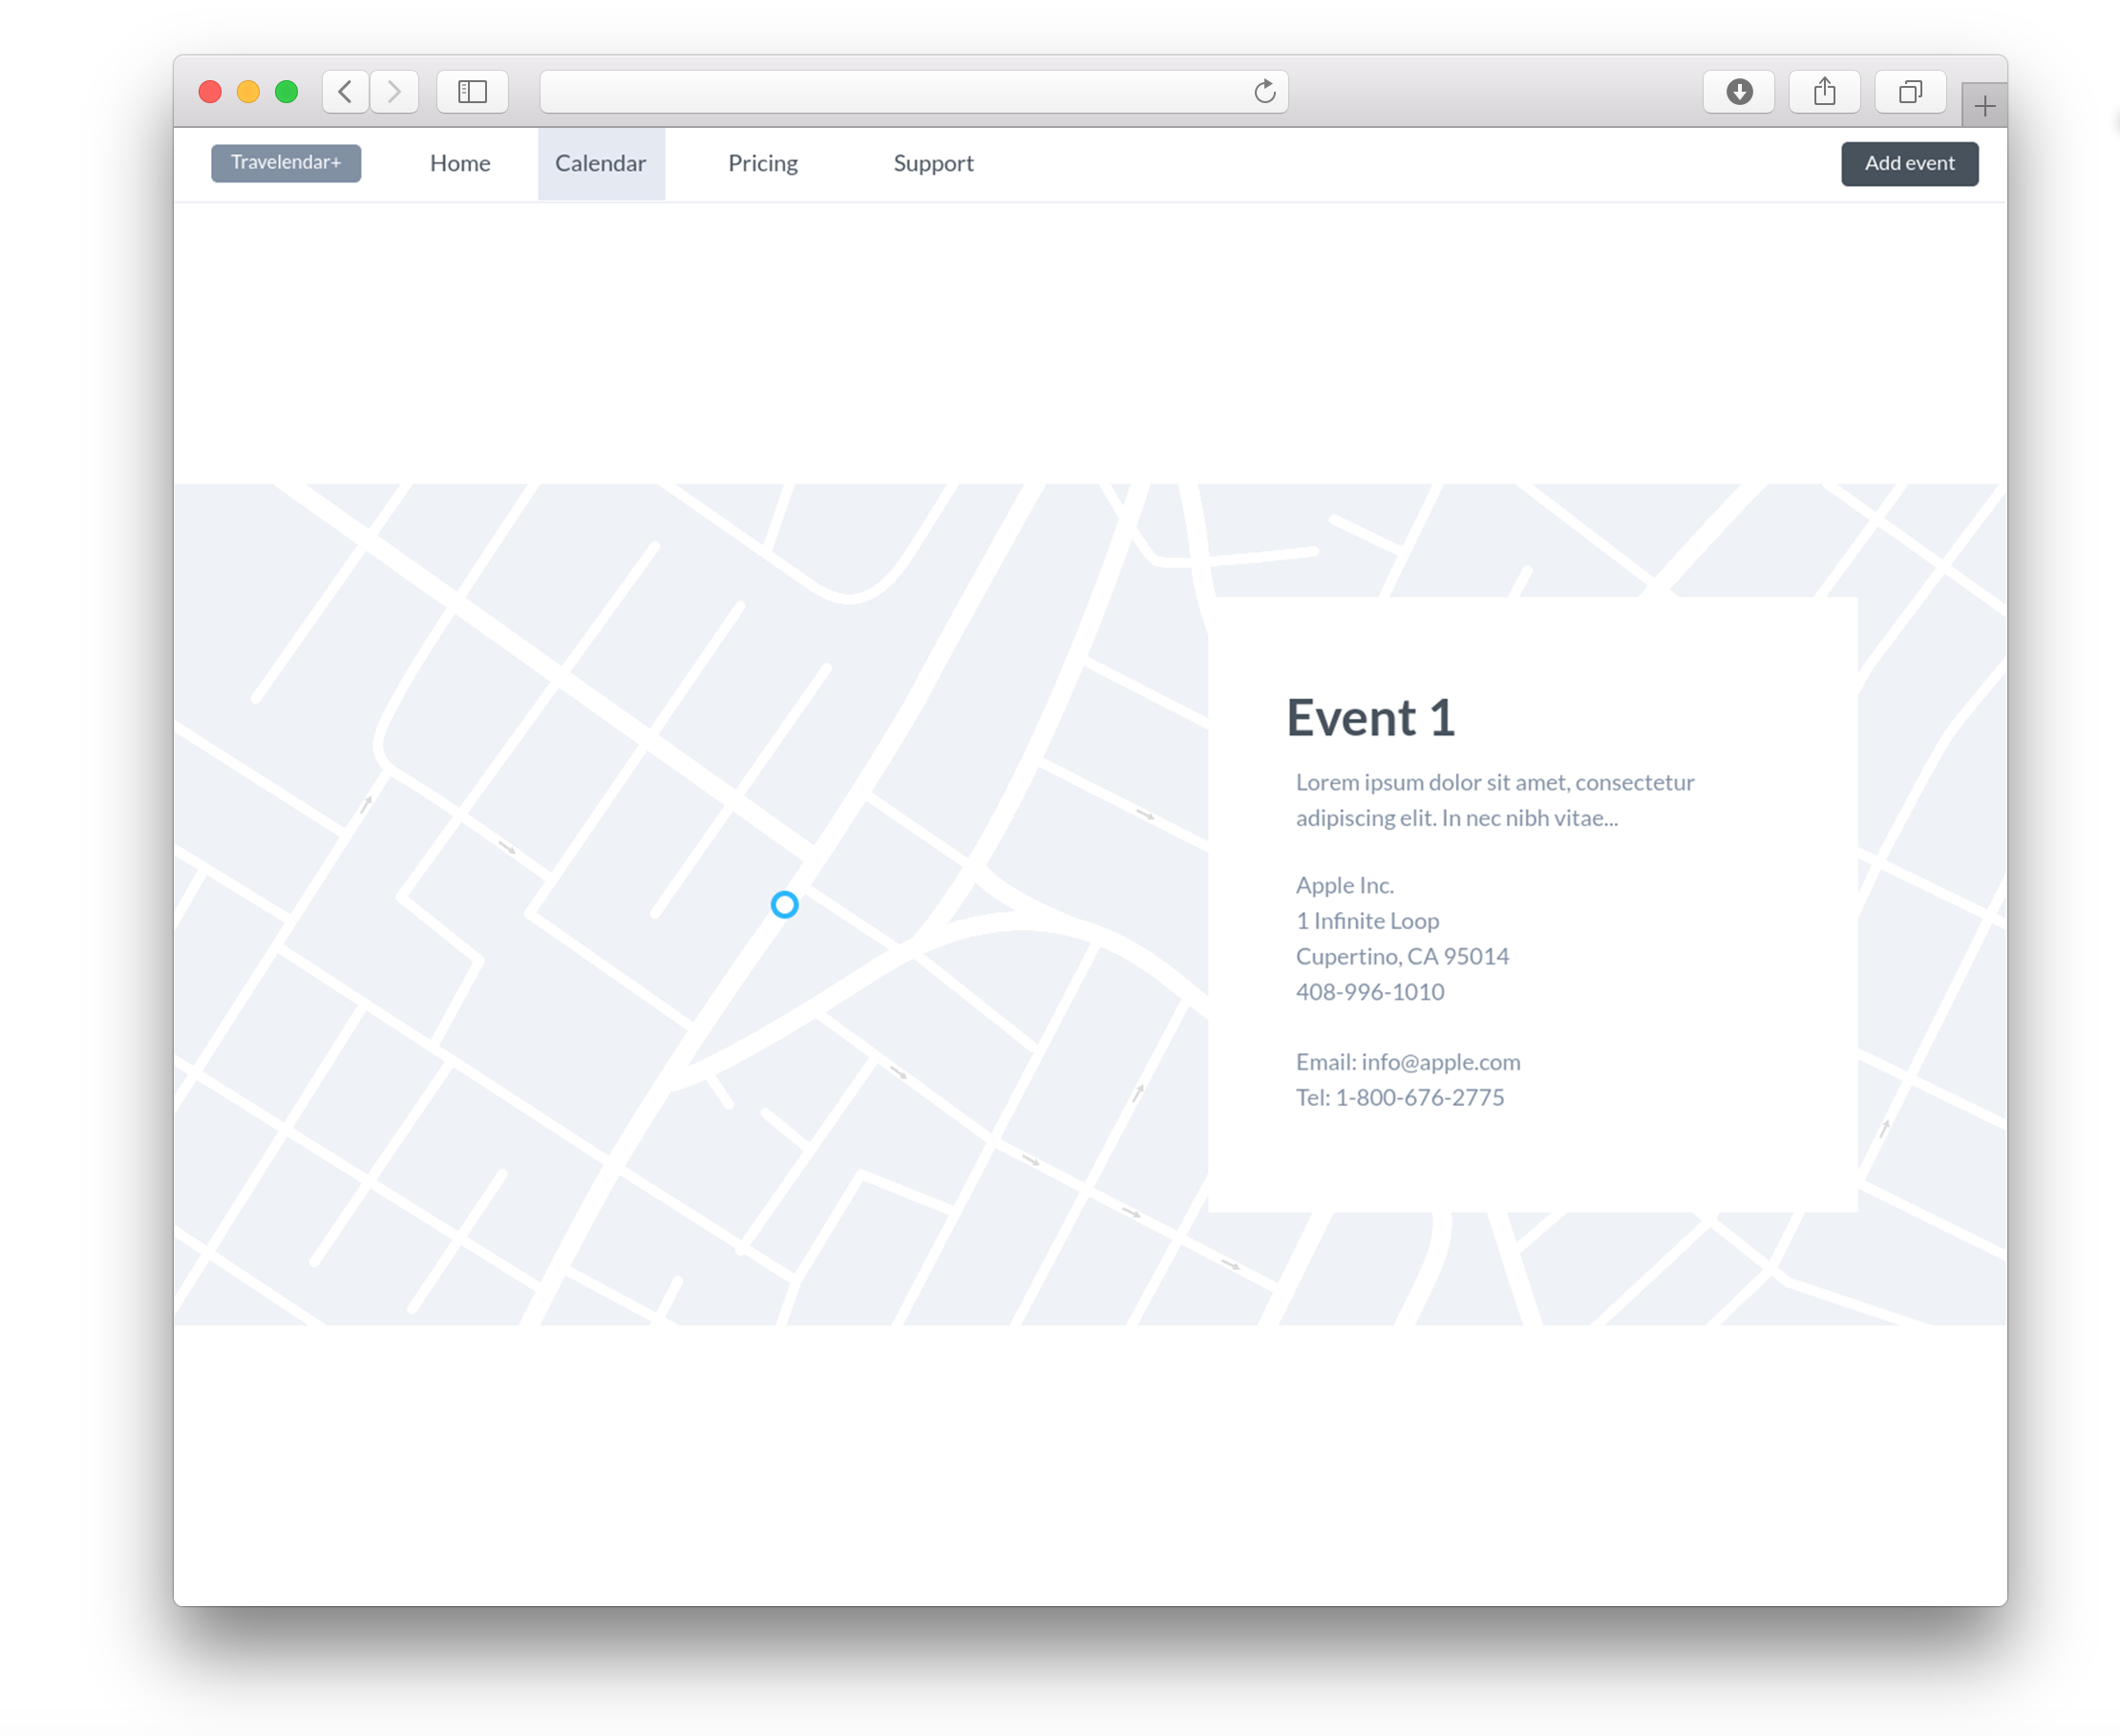
\includegraphics[scale=0.25]{img/mockups/web/map.png}
		\caption{Mockup for meetings map view on a browser.}
	\end{figure}


	\newpage
	\subsubsection{Delete meetings}
	
	\bigskip
	\noindent
	\textbf{Purpose} \\
	The purpose of this part is to allow the user, after creating or modifying an meeting on the calendar, to delete it.
	
	\bigskip
	\noindent
	\textbf{Scenario 1} \\
	Igor is a computer science student. He attends on Monday and Tuesday the course  Database 2. The professor has just written an email, signaling that on next Monday there will be no lesson. Igor opens the "Travlendar +" application on his smartphone and he logs in. He selects the "DB2 lesson" meeting and clicks on “Delete” button. The system asks whether he is sure to cancel the meeting. Igor confirms. The system processes the information and updates the database.
	
	\bigskip
	\noindent
	\textbf{Use cases} \\
	
	\begin{center}
		Table 3.5: Delete meetings use case.
		
		\bigskip
    		\begin{tabular}{p{0.3\textwidth}|p{0.6\textwidth}}
   		 	\hline
    			Actor & User \\ \hline
    			Goal & Goal 6 \\ \hline
    			Input Condition & The user wants to delete a meeting on his/her calendar. \\ \hline
    			Event flow & 
			\begin{enumerate}
  				\item The user must login entering your email and password;
  				\item The user selects the meeting he/she wants to select with one click;
  				\item The system shows a dialog box with two buttons: "Modify" and "Delete";
  				\item The user clicks on "Delete" button;
  				\item The system prompts the user if he/she is sure and wants to delete the meeting with a dialog box;
  				\item The user presses on "Yes" button;
  				\item The system processes the information, updates the database, and deletes the event from the calendar.
 			 \end{enumerate} \\ \hline
    			Output Condition & The system deletes a meeting on the user's home calendar. \\ \hline
    			Exception & The delete fails and the user is notified. \\ \hline
    		\end{tabular}
	\end{center}
	
	\bigskip
	\noindent
	\textbf{Functional requirements} \\
	\begin{itemize}
		\item The user must log in successfully;
		\item The user must have already created a meeting;
		\item The user must select the meeting he/she wants to delete;
		\item The system must ask the user whether or not he/she wants to delete the meeting;
		\item The system must update the DB and delete the meeting from the calendar.
	\end{itemize}
	
	\newpage
	\noindent
	\textbf{Activity diagram} \\
	
	\begin{figure}[h!]
		\bigskip
		\centering
		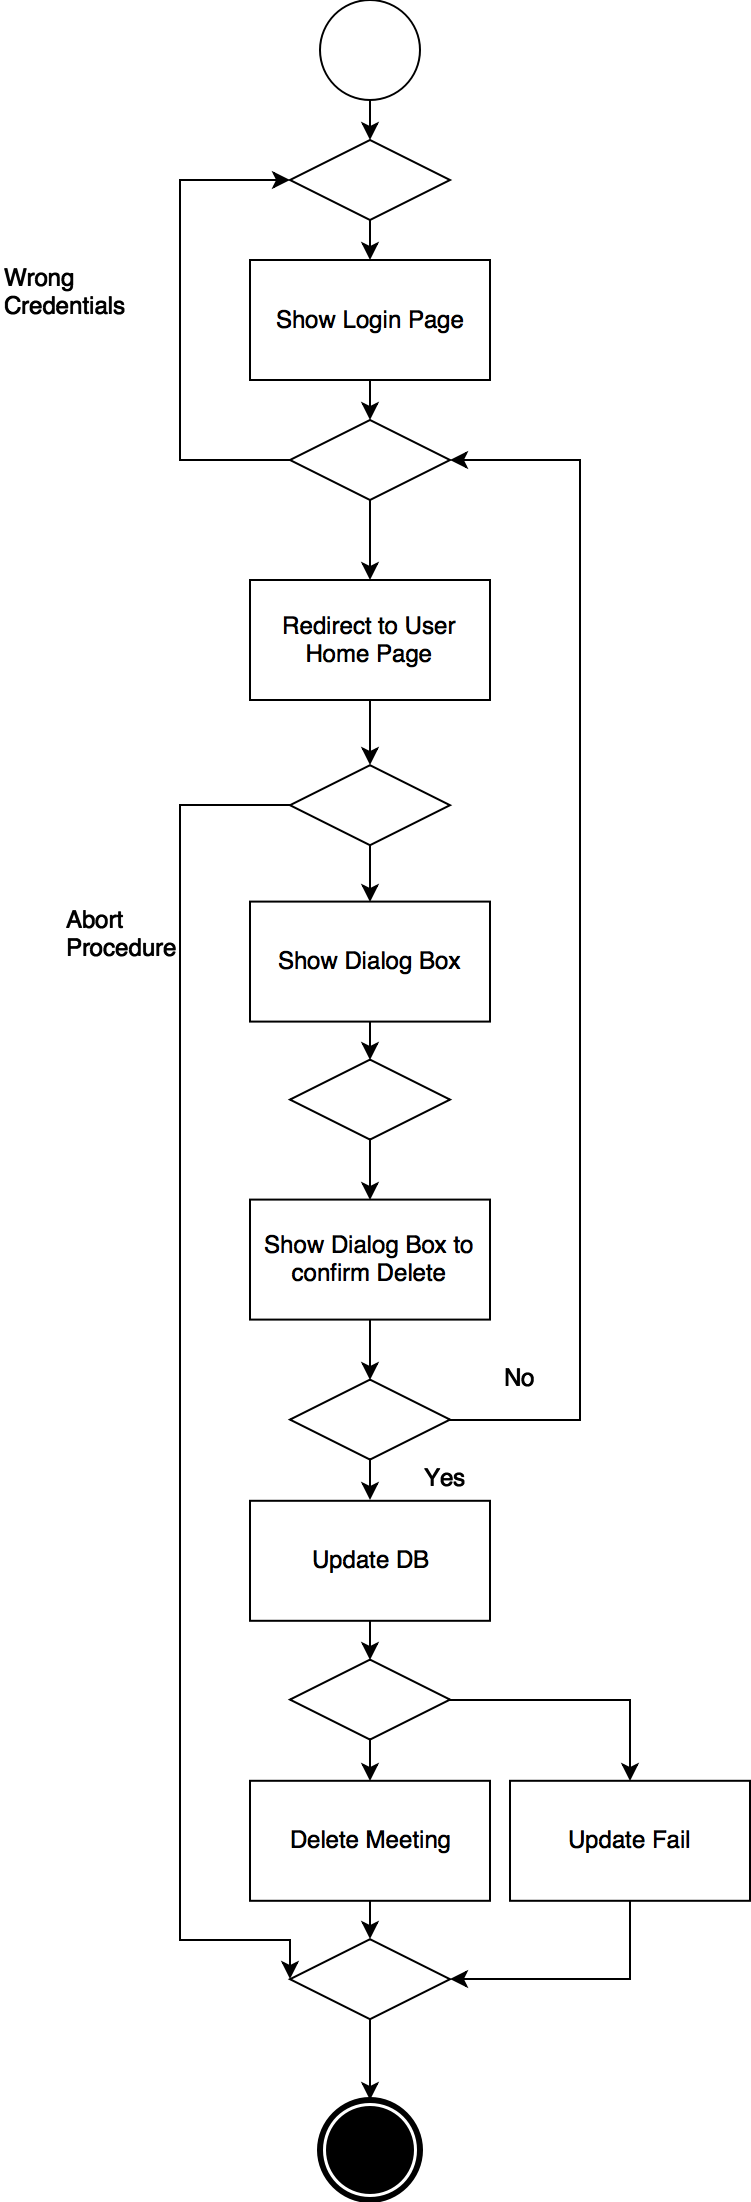
\includegraphics[scale=0.25]{img/diagrams/delete_meetings_ad.png}
		\caption{Activity diagram for Delete meetings.}
	\end{figure}
	\newpage

	\subsubsection{Manage profile informations}
	
	\bigskip
	\noindent
	\textbf{Purpose} \\
	Both web and mobile applications must allow the user to view and update some personal informations coherently with the provided constraints.
	
	\bigskip
	\noindent
	\textbf{Scenario 1} \\
	Karlie, due to a problem with her e-mail services provider, wants to change her email address. Karlie opens a browser window, reaches the Travelendar+ homepage and logs in. Then she clicks on her profile picture in the right of the navigation bar, a dropdown menu appears and clicking "Edit Profile" she reaches a page showing her profile information. She changes her email address and clicks then on "Save Changes" button. The system notifies Karlie that her email address has been correctly updated.
	
	\bigskip
	\noindent
	\textbf{Use cases} \\
	
	\begin{center}
		Table 3.6: Manage profile informations use case.
		
		\bigskip
   		\begin{tabular}{p{0.3\textwidth}|p{0.6\textwidth}}
   		 	\hline
    			Actor & User \\ \hline
    			Goal & Goal 2 \\ \hline
    			Input Condition & A user wants to view or update his/her personal informations. \\ \hline
    			Event flow & 
			\begin{enumerate}
  				\item The user opens a web browser page or the mobile application and, if he/she has not already done it, authenticates to the service;
  				\item The user reaches his/her profile settings page;
  				\item The user updates his/her personal information.
 			 \end{enumerate} \\ \hline
    			Output Condition & Information concerning the user is successfully updated and the user is notified. \\ \hline
    			Exception & The update fails and the user is notified.\\
    			\hline
    		\end{tabular}
	\end{center}
	
	\bigskip
	\noindent
	\textbf{Functional requirements} \\
	\begin{itemize}
		\item The user must be already logged in;
		\item The system must display to the user his/her own personal informations;
		\item The system must allow the user to change any information provided during the registration phase, only if the new piece of information does not get in conflict with the registration constrains;
		\item Either a modification succeeds or it fails, the user must be notified.
	\end{itemize}
	
	\newpage
	\noindent
	\textbf{Activity diagram} \\
	
	\begin{figure}[h!]
		\bigskip
		\centering
		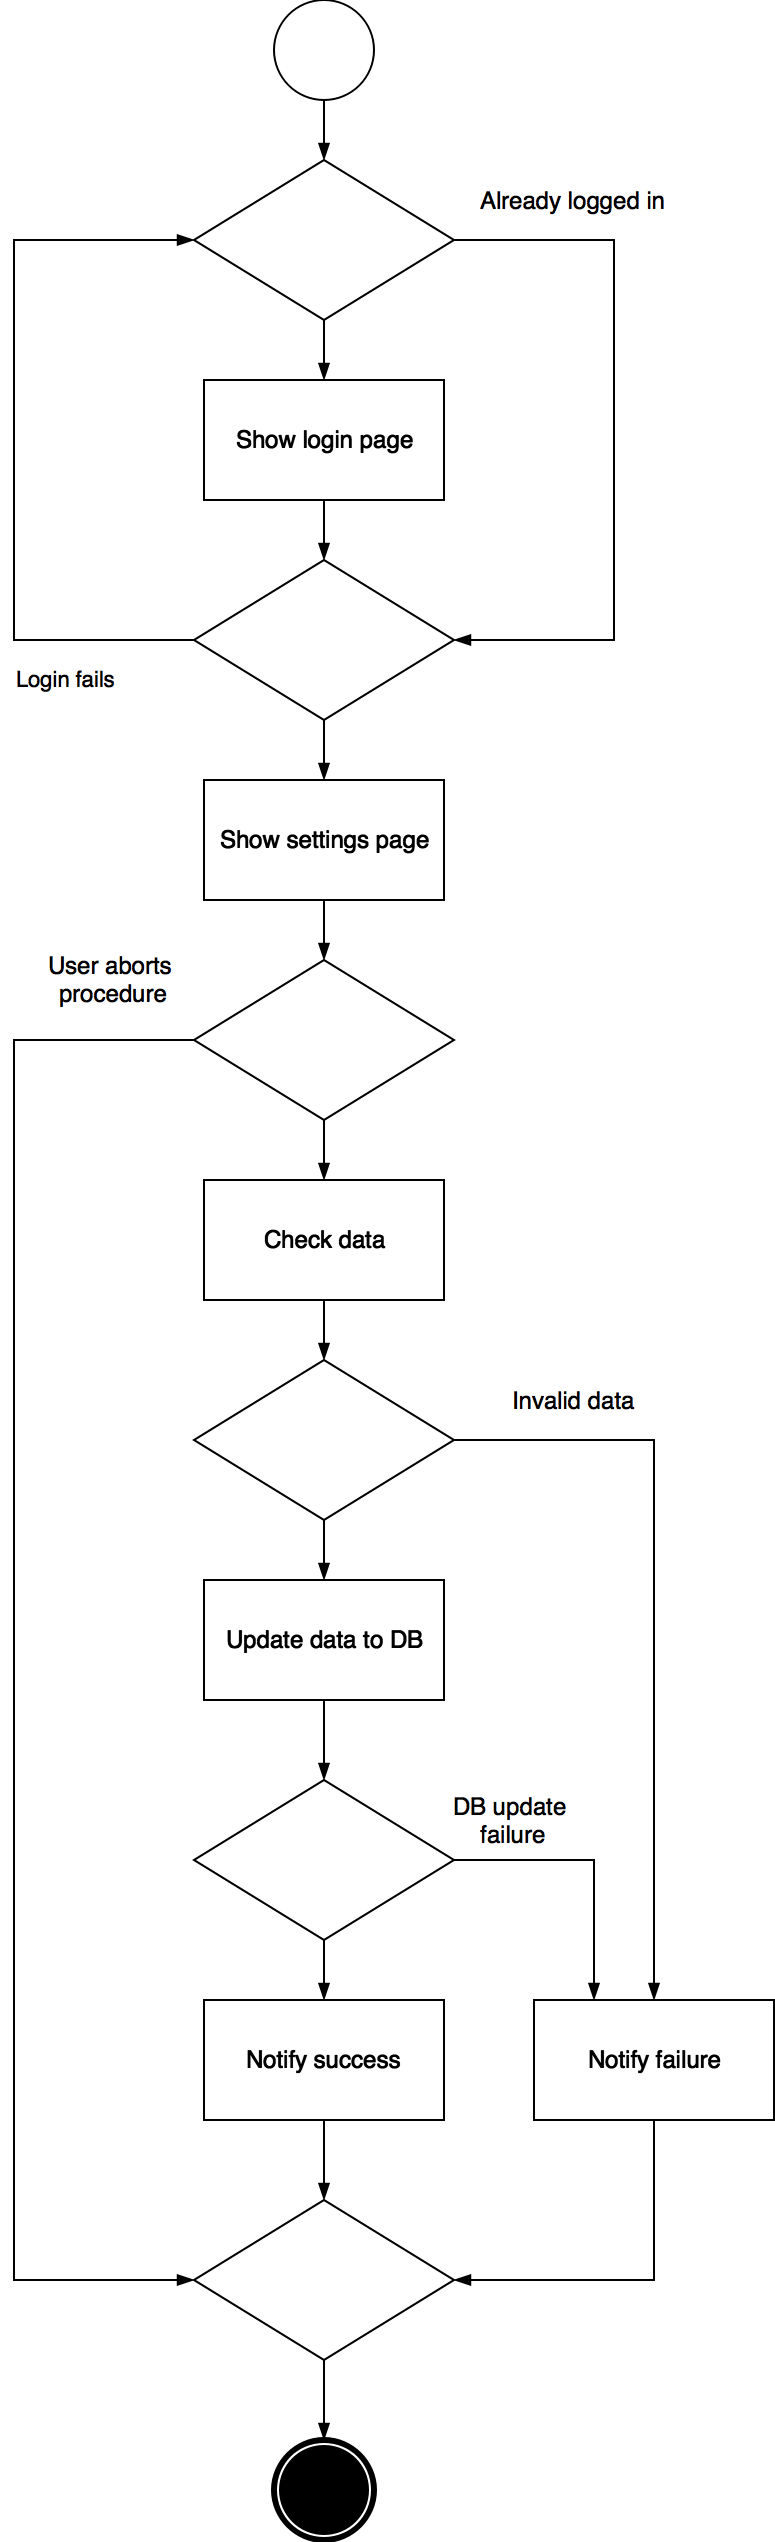
\includegraphics[scale=0.23]{img/diagrams/manage_profile_informations_ad.png}
		\caption{Activity diagram for Manage profile informations.}
	\end{figure}


	\subsubsection{Delete profile}
	
	\bigskip
	\noindent
	\textbf{Purpose} \\
	Both web and mobile applications must allow the user to delete his/her account if does no longer want to use the service.
	
	\bigskip
	\noindent
	\textbf{Scenario 1} \\
	Luca decides that he no longer wants to use Travelendar+ and wants to delete his account. Luca opens the mobile application and clicks the profile button on the navigation bar, the profile informations page is now displayed. He clicks on the red button "Delete Account". As soon as and after he confirms his intentions, Luca is no longer a Travelendar+ registered user and  his data are no longer stored in the system.
	
	\bigskip
	\noindent
	\textbf{Use cases} \\
	
	\begin{center}
		Table 3.7: Delete profile use case.
		
		\bigskip
    			\begin{tabular}{p{0.3\textwidth}|p{0.6\textwidth}}
   		 	\hline
    			Actor & User \\ \hline
    			Goal & Goal 3 \\ \hline
    			Input Condition & An user wants to delete his/her account. \\ \hline
    			Event flow & 
			\begin{enumerate}
  				\item The user opens a web browser page or the mobile application and, if he/she has not already done it, authenticates to the service;
  				\item The user reaches his/her profile settings page;
  				\item The user clicks on "Delete account" button;
  				\item The user confirms his/her intent to delete the account.
 			 \end{enumerate} \\ \hline
    			Output Condition & The user’s account is deleted, his/her data are erased from the system and of course he/she can no longer login with his/her credentials, unless he/she registers into the service again. \\ \hline
    			Exception & The account's deletion fails and the user is notified. \\
    			\hline
    		\end{tabular}
	\end{center}
	
	\bigskip
	\noindent
	\textbf{Functional requirements} \\
	\begin{itemize}
		\item The user must be already logged in;
		\item The system must allow the user to delete his/her profile;
		\item The user must confirm his/her intention to delete his/her profile;
		\item Once the user's profile has been deleted, the system must no longer store the user's personal informations.
		\item Once the user’s profile has been deleted, the user can no longer login with his/her credentials unless he/she re-register to the service;
		\item Either a modification succeeds or it fails, the user must be notified.
	\end{itemize}
	
	\newpage
	\noindent
	\textbf{Activity diagram} \\
	
	\begin{figure}[h!]
		\bigskip
		\centering
		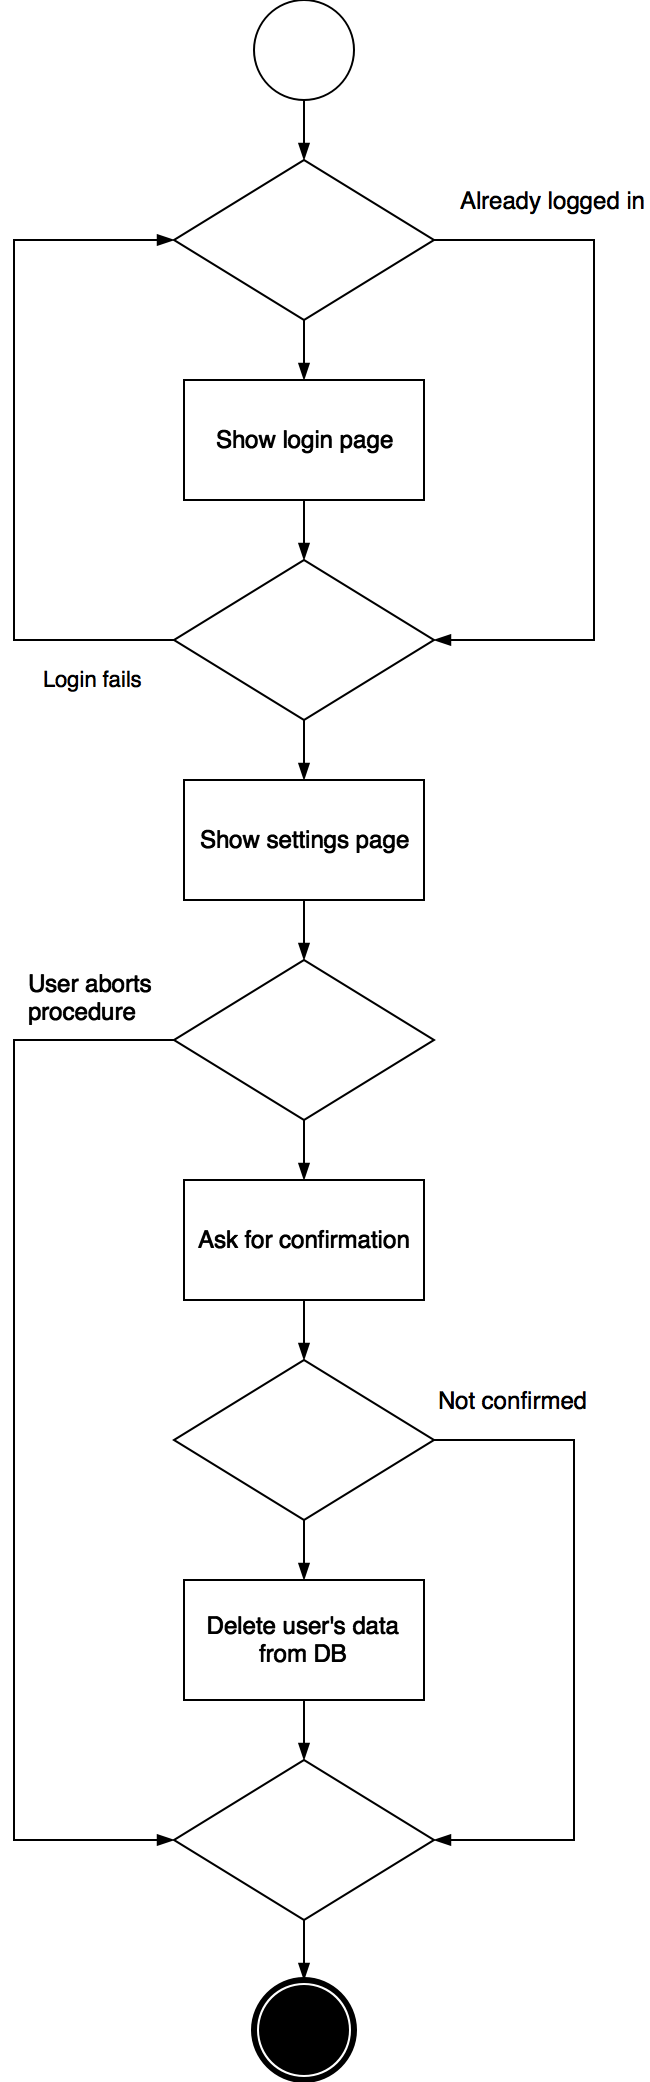
\includegraphics[scale=0.25]{img/diagrams/delete_profile_ad.png}
		\caption{Activity diagram for Delete profile.}
	\end{figure}
	\newpage
	

	\subsubsection{Activate travel mean(s)}
	
	\bigskip
	\noindent
	\textbf{Purpose} \\
	Both web and mobile applications must allow the user to specify his/her intention to use a specific travel mean to move from an event to another.
	
	\bigskip
	\noindent
	\textbf{Scenario 1} \\
	It’s almost summer. Mario decides that the weather is good enough to allow him to use the bike. Mario opens the Travelendar+ app on his Android smartphone and navigates to the settings page, scrolls down until he reaches "Bike" in the travel menas list and toggles the checkbox near to it. From now on the system will also suggest him the bike as an appropriate mean of transport, if it thinks it is appropriate.
	
	\bigskip
	\noindent
	\textbf{Use cases} \\
	
	\begin{center}
		Table 3.8: Activate travel mean(s) use case.
		
		\bigskip
    		\begin{tabular}{p{0.3\textwidth}|p{0.6\textwidth}}
   		 	\hline
    			Actor & User \\ \hline
    			Goal & Goal 9 \\ \hline
    			Input Condition & The user wants to activate a travel mean. \\ \hline
    			Event flow & 
			\begin{enumerate}
  				\item The user opens a web browser page or the mobile application and, if he/she has not already done it, authenticates to the service;
  				\item The user reaches his/her profile settings page;
  				\item The user checks the checkbox corresponding to the travel mean he/she wants to activate.
 			 \end{enumerate} \\ \hline
    			Output Condition & The travel mean(s) is/are now activated as desired; the user is notified about it. \\ \hline
    			Exception & The travel mean(s) activation fails and the user is notified. \\ \hline
    		\end{tabular}
	\end{center}
	
	\bigskip
	\noindent
	\textbf{Functional requirements} \\
	\begin{itemize}
		\item The user must be already logged in;
		\item The system must display to the user which travel mean is already selected;
		\item The system must allow the user to select a travel mean if it was not already selected;
		\item If a new travel mean has been selected, from now on it must the system take it into consideration when it calculates the more convenient travel between the two locations;
		\item Either a modification succeeds or it fails, the user must be notified.
	\end{itemize}
	
	\newpage
	\noindent
	\textbf{Activity diagram} \\
	
	\begin{figure}[h!]
		\bigskip
		\centering
		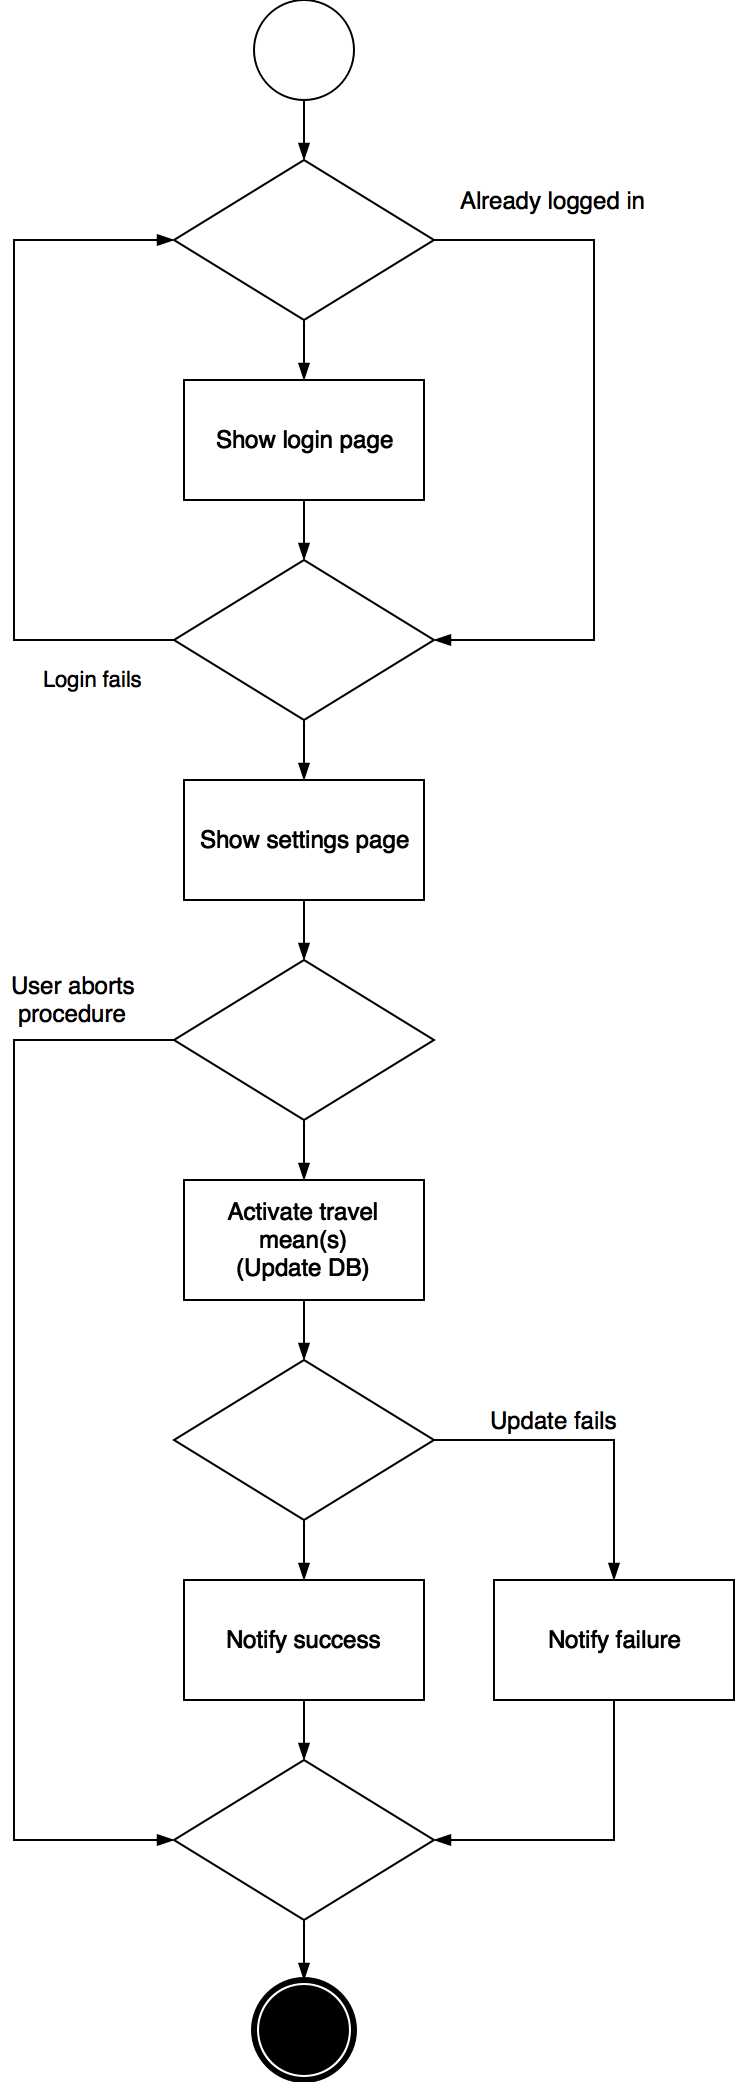
\includegraphics[scale=0.25]{img/diagrams/activate_travel_mean_ad.png}
		\caption{Activity diagram for Activate travel mean(s).}
	\end{figure}
	\newpage

	\subsubsection{Deactivate travel mean(s)}
	
	\bigskip
	\noindent
	\textbf{Purpose} \\
	Both web and mobile applications must allow the user to specify his/her intention to do not use a specific travel mean to move from an event to another.
	
	\bigskip
	\noindent
	\textbf{Scenario 1} \\
	Otis, after breaking his leg, realizes that the only suitable means for his travels are taxi and Uber. Otis opens a browser window, reaches the Travelendar+ homepage and logs in. Then he clicks on his profile picture in the right of navigation bar, a dropdown menu appears and clicking "Edit Profile" he reaches a page showing his profile information and unchecks all the checkboxes near to the travel means excepted, either "Taxi" or "Uber". From now on the system could only rely on one other travel mean, either Taxi or Uber.
	
	\bigskip
	\noindent
	\textbf{Use cases} \\
	
	\begin{center}
		Table 3.9: Deactivate travel mean(s) use case.
		
		\bigskip
    		\begin{tabular}{p{0.3\textwidth}|p{0.6\textwidth}}
   		 	\hline
    			Actor & User \\ \hline
    			Goal & Goal 9 \\ \hline
    			Input Condition & The user wants to deactivate a travel mean. \\ \hline
    			Event flow & 
			\begin{enumerate}
  				\item The user opens a web browser page or the mobile application and, if he/she has not already done, authenticates to the service;
  				\item The user reaches his/her profile settings page;
  				\item The user unchecks the checkbox corresponding to the travel mean he/she wants to deactivate.
 			 \end{enumerate} \\ \hline
    			Output Condition & The travel mean(s) is/are now deactivated as desired and the user is notified. \\ \hline
    			Exception & The travel mean(s) deactivation fails and the user is notified. \\ \hline
    		\end{tabular}
	\end{center}
	
	\bigskip
	\noindent
	\textbf{Functional requirements} \\
	\begin{itemize}
		\item The user must be already logged in;
		\item The system must display the user travel mean already selected;
		\item The system must allow the user to deselect a travel mean if it was not previously selected;
		\item If a travel mean has been deselected, from now on it can not be taken in consideration when the system calculates the optimal travel between two locations;
		\item Either a modification succeeds or it fails, the user must be notified.
	\end{itemize}
	
	\newpage
	\noindent
	\textbf{Activity diagram} \\
	
	\begin{figure}[h!]
		\bigskip
		\centering
		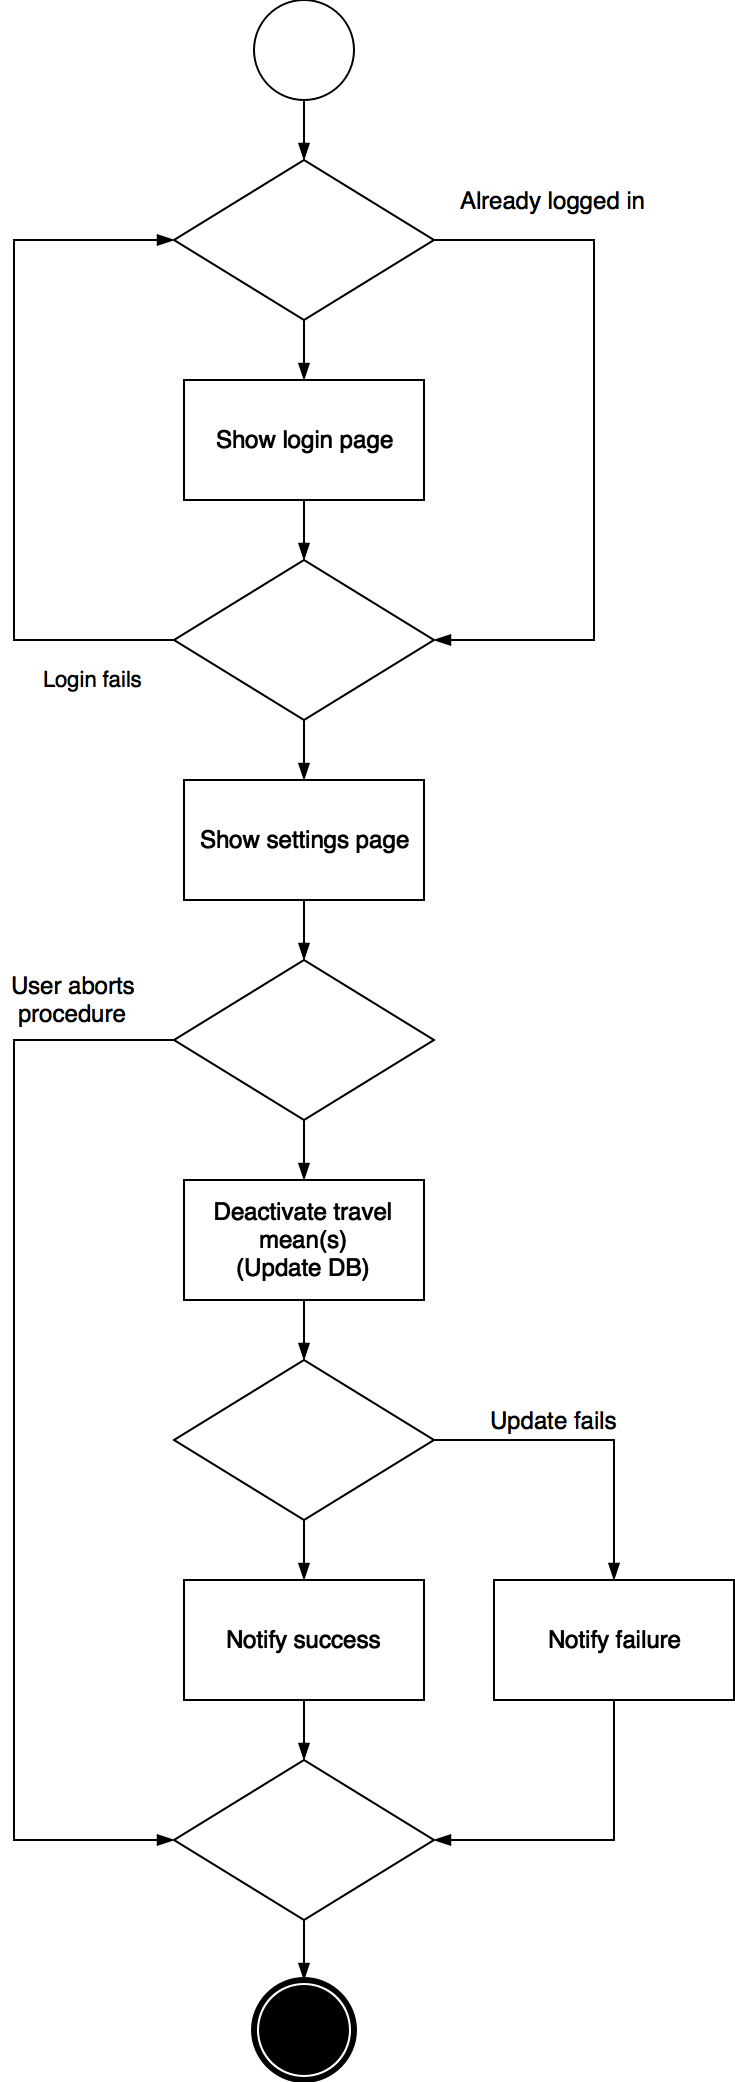
\includegraphics[scale=0.25]{img/diagrams/deactivate_travel_mean_ad.png}
		\caption{Activity diagram for Deactivate travel mean(s).}
	\end{figure}
	\newpage
	

	\subsubsection{Provide constraints}
	
	\bigskip
	\noindent
	\textbf{Purpose} \\
	Both web and mobile applications must allow the user to select a specific travel mean for a specific travel.
	
	\bigskip
	\noindent
	\textbf{Scenario 1} \\
	Quentin has a meeting scheduled for tomorrow morning at 9:00AM not far away from his house. The system suggests him to take the bus, but Quentin needs to take to the meeting a cumbersome model of the building he will present to his boss. Due to his particular need he decides that the most appropriate transport mean is a taxi. He opens the Travelendar+ app on his iPhone. In the page detailing events, he selects the taxi as the preferred mean of transport and the system re-calculates the travel time and eventually reserves a vehicle for the next morning.
	
	\bigskip
	\noindent
	\textbf{Use cases} \\
	
	\begin{center}
		Table 3.10: Provide constraints use case.
		
		\bigskip
  		\begin{tabular}{p{0.3\textwidth}|p{0.6\textwidth}}
   		 	\hline
    			Actor & User \\ \hline
    			Goal & Goal 8 \\ \hline
    			Input Condition & The user wants to select a specific travel mean for a specific travel. \\ \hline
    			Event flow & 
			\begin{enumerate}
  				\item The user opens a web browser page or the mobile application and, if he/she has not already done it, authenticates to the service;
  				\item The user opens the detail page of a certain event;
  				\item The user selects a certain travel mean, the one he/she prefers for travelling.
 			 \end{enumerate} \\ \hline
    			Output Condition & The change succeeded and the mean for that travel is updated. \\ \hline
    			Exception & The change fails and the user is notified. \\ \hline
    		\end{tabular}
	\end{center}
	
	\bigskip
	\noindent
	\textbf{Functional requirements} \\
	\begin{itemize}
		\item The user must be already logged in;
		\item The system must allow the user to use a specific travel mean to reach a given event (only if the mean can reach the event's location);
		\item Either a modification succeeds or it fails, the user must be notified.
	\end{itemize}
	
	\newpage
	\noindent
	\textbf{Activity diagram} \\
	
	\begin{figure}[h!]
		\bigskip
		\centering
		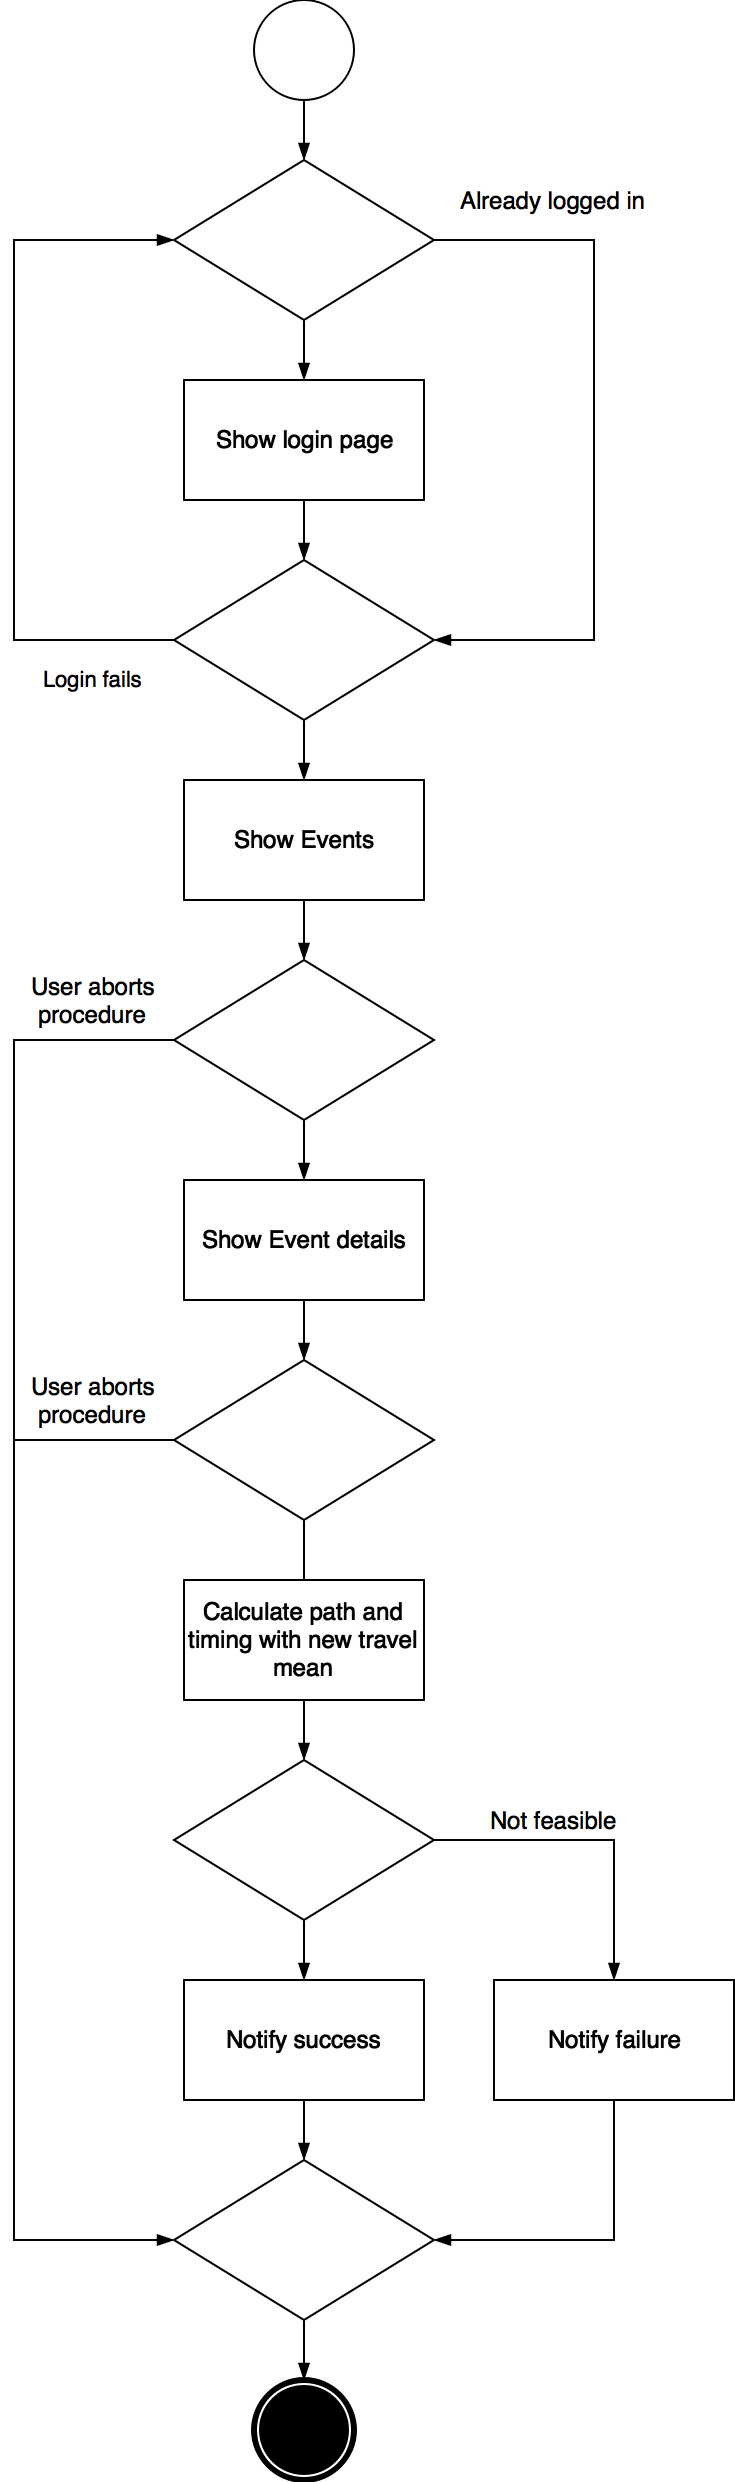
\includegraphics[scale=0.23]{img/diagrams/provide_constraints_ad.png}
		\caption{Activity diagram for Provide constraints.}
	\end{figure}


	\subsubsection{Minimize carbon footprint}
	
	\bigskip
	\noindent
	\textbf{Purpose} \\
	Both web and mobile applications must allow the user to specify his/her intention to move from an appointment to another with the less polluting mean(s).
	
	\bigskip
	\noindent
	\textbf{Scenario 1} \\
	Serena, while she was watching a National Geographic documentary, realized that climate change is a real thing and everyone should do his best to limit pollution. For this reason she wants to minimize her carbon footprint during her travels. Serena opens a browser window, reaches the Travelendar+ homepage and logs in. Then she clicks on her profile picture in the right of navigation bar, a dropdown menu appears and by clicking "Edit Profile" she reaches a page showing her profile information and toggles the checkbox near to "Minimize carbon footprint". From now on the suggested travel mean is the less polluting one.
	
	\bigskip
	\noindent
	\textbf{Use cases} \\
	
	\begin{center}
		Table 3.11: Minimize carbon footprint use case.
		
		\bigskip
   		\begin{tabular}{p{0.3\textwidth}|p{0.6\textwidth}}
   		 	\hline
    			Actor & User \\ \hline
    			Goal & Goal 12 \\ \hline
    			Input Condition & The user wants to move from an appointment to another with the less polluting mean(s). \\ \hline
    			Event flow & 
			\begin{enumerate}
  				\item The user opens a web browser page or the mobile application and, if he/she has not already done it, authenticates to the service;
				\item The user reaches his/her profile settings page;
				\item The user checks the checkbox corresponding to "Minimize carbon footprint".
 			 \end{enumerate} \\ \hline
    			Output Condition & The preference update succeeds and the user is notified. \\ \hline
    			Exception & The preference update fails and the user is notified. \\ \hline
    		\end{tabular}
	\end{center}
	
	\bigskip
	\noindent
	\textbf{Functional requirements} \\
	\begin{itemize}
		\item The user must be already logged in;
		\item The system must allow the user to express his/her intention to minimize his/her carbon footprint or not;
		\item If the user has expressed the intention to minimize his/her carbon footprint, the suggested travel mean must be the less polluting one;
		\item Either a modification succeeds or it fails, the user must be notified.
	\end{itemize}
	
	\newpage
	\noindent
	\textbf{Activity diagram} \\
	
	\begin{figure}[h!]
		\bigskip
		\centering
		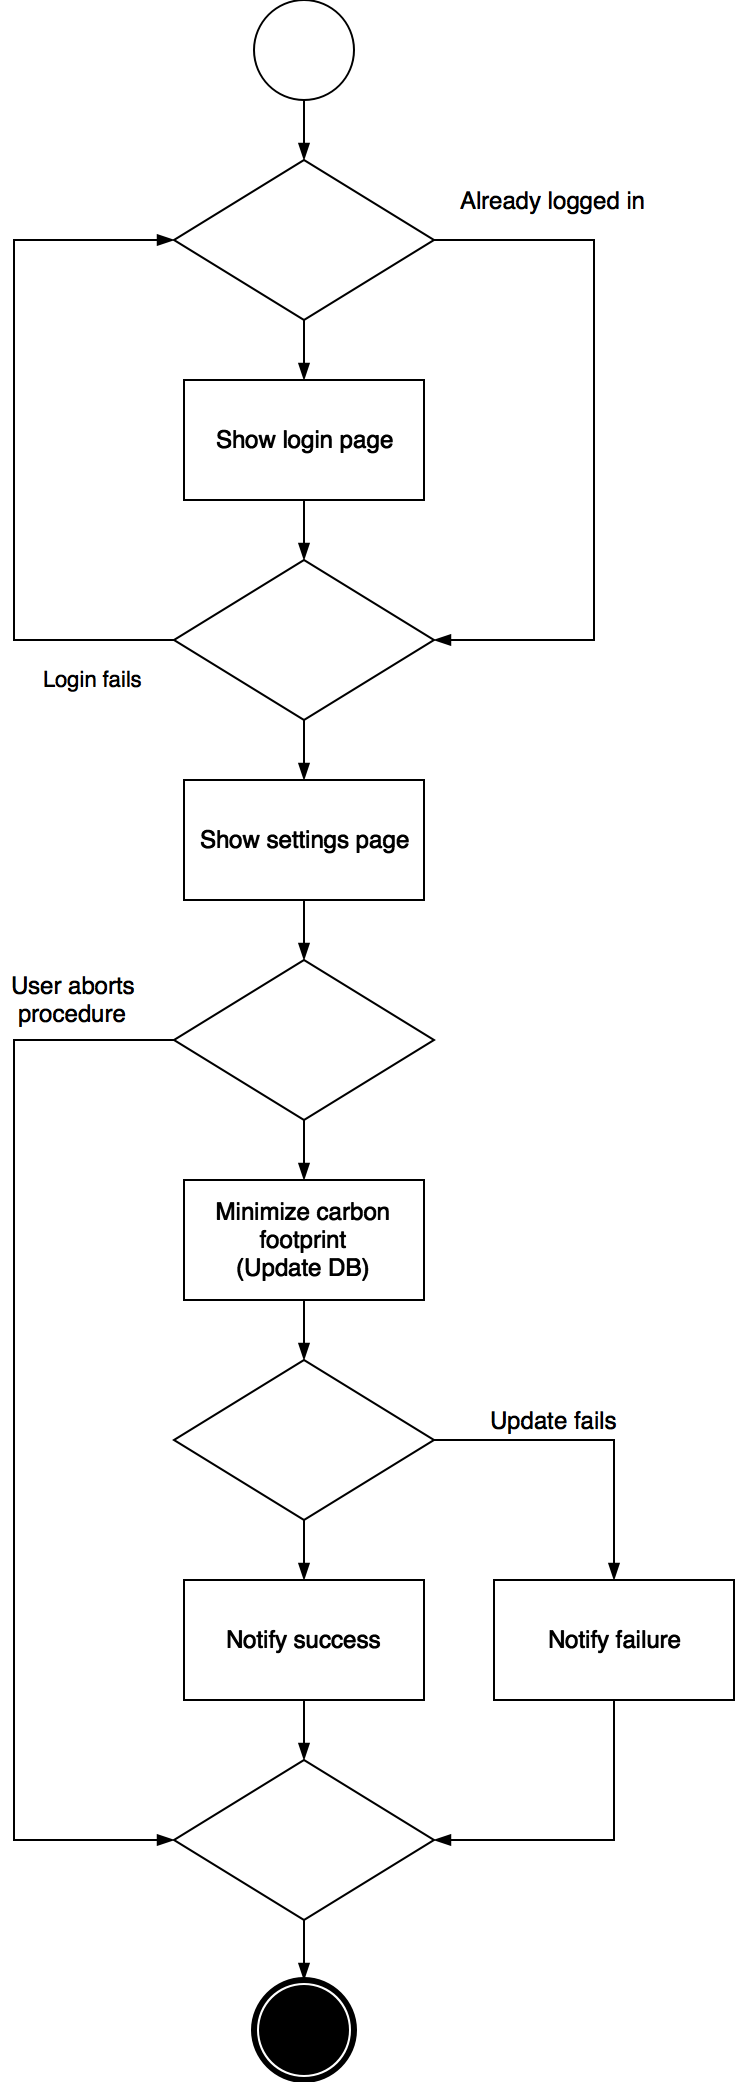
\includegraphics[scale=0.25]{img/diagrams/minimize_carbon_footprint_ad.png}
		\caption{Activity diagram for Minimize carbon footprint.}
	\end{figure}
	\newpage


	\subsubsection{Specify break timing}
	
	\bigskip
	\noindent
	\textbf{Purpose} \\
	The purpose is to allow the user to enter a time interval where the system must ensure at least half an hour for the break, based on the present appointments.
	
	\bigskip
	\noindent
	\textbf{Scenario 1} \\
	Ubald is a university professor and on Wednesday he has two hours lesson in the morning (10 a.m. -- 12 a.m.) and two hours lesson in the afternoon (1 p.m. –-- 3 p.m.). Ubald connects to the "Travlendar +" home page and selects the "BreakTime" entry. The system shows you a form to be filled in with the date and time interval for the break. Ubald inserts the break  from 12.30 to 15.30 and submits it by pressing on "Save". The system verifies availability and saves it successfully in the database.
	
	\bigskip
	\noindent
	\textbf{Scenario 2} \\
	Vichy is a manager who has to go to Naples for a meeting at 3:15 p.m.. She bought a train ticket from Milan at 10.30 a.m.. The journey lasts 270 minutes. Vichy opens the mobile application of "Travlendar +" and selects the entry "BreakTime". The system shows a form to be filled in with the date and duration for the break. Vichy inserts as interval 1 p.m. -- 3 p.m. and submits it pressing on"Save" button. The system checks the information and sends an error message.
	
	\bigskip
	\noindent
	\textbf{Use cases} \\
	
	\begin{center}
		Table 3.12: Specify lunch timing use case.
		
		\bigskip
    		\begin{tabular}{p{0.3\textwidth}|p{0.6\textwidth}}
   		 	\hline
    			Actor & User \\ \hline
    			Goal & Goal 13 and Goal 14 \\ \hline
    			Input Condition & The user specifies a time interval for break. \\ \hline
    			Event flow & 
			\begin{enumerate}
  				\item The user must login entering his/her email and password.;
  				\item The user selects "Break Time" button;
  				\item The system opens a form to be completed indicating date and duration of the interval;
  				\item The user inserts information regarding the date and the duration of break;
  				\item The user saves the information pressing on "Save" button;
  				\item The system processes the information, updates the database and notifies the user that the operation has been successfully concluded (specifying the start and end time for break). If not, it generates an error message.
 			 \end{enumerate} \\ \hline
    			Output Condition & The system selects within the time interval, time of specify duration for the break. \\ \hline
    			Exception & The system issues an error message if there is no duration time for the break during the specified time interval. \\ \hline
    		\end{tabular}
	\end{center}
	
	\bigskip
	\noindent
	\textbf{Functional requirements} \\
	\begin{itemize}
		\item The user must log in successfully.
		\item The user must enter information in the form:
			\begin{itemize}
				\item Start at least
				\item End at most
				\item Duration
			\end{itemize}
		\item The system must verify that the date is behind the insertion date.
		\item The system must check that the available time (duration time) is sufficient for the break.
		\item Once the information are verified, the system must update the database.
		\item The system must alert the user about the selected time interval.
		\item The system must send an error message if an incorrect date or time space is not available.
	\end{itemize}
	
	\newpage
	\noindent
	\textbf{Activity diagram} \\
	
	\begin{figure}[h!]
		\bigskip
		\centering
		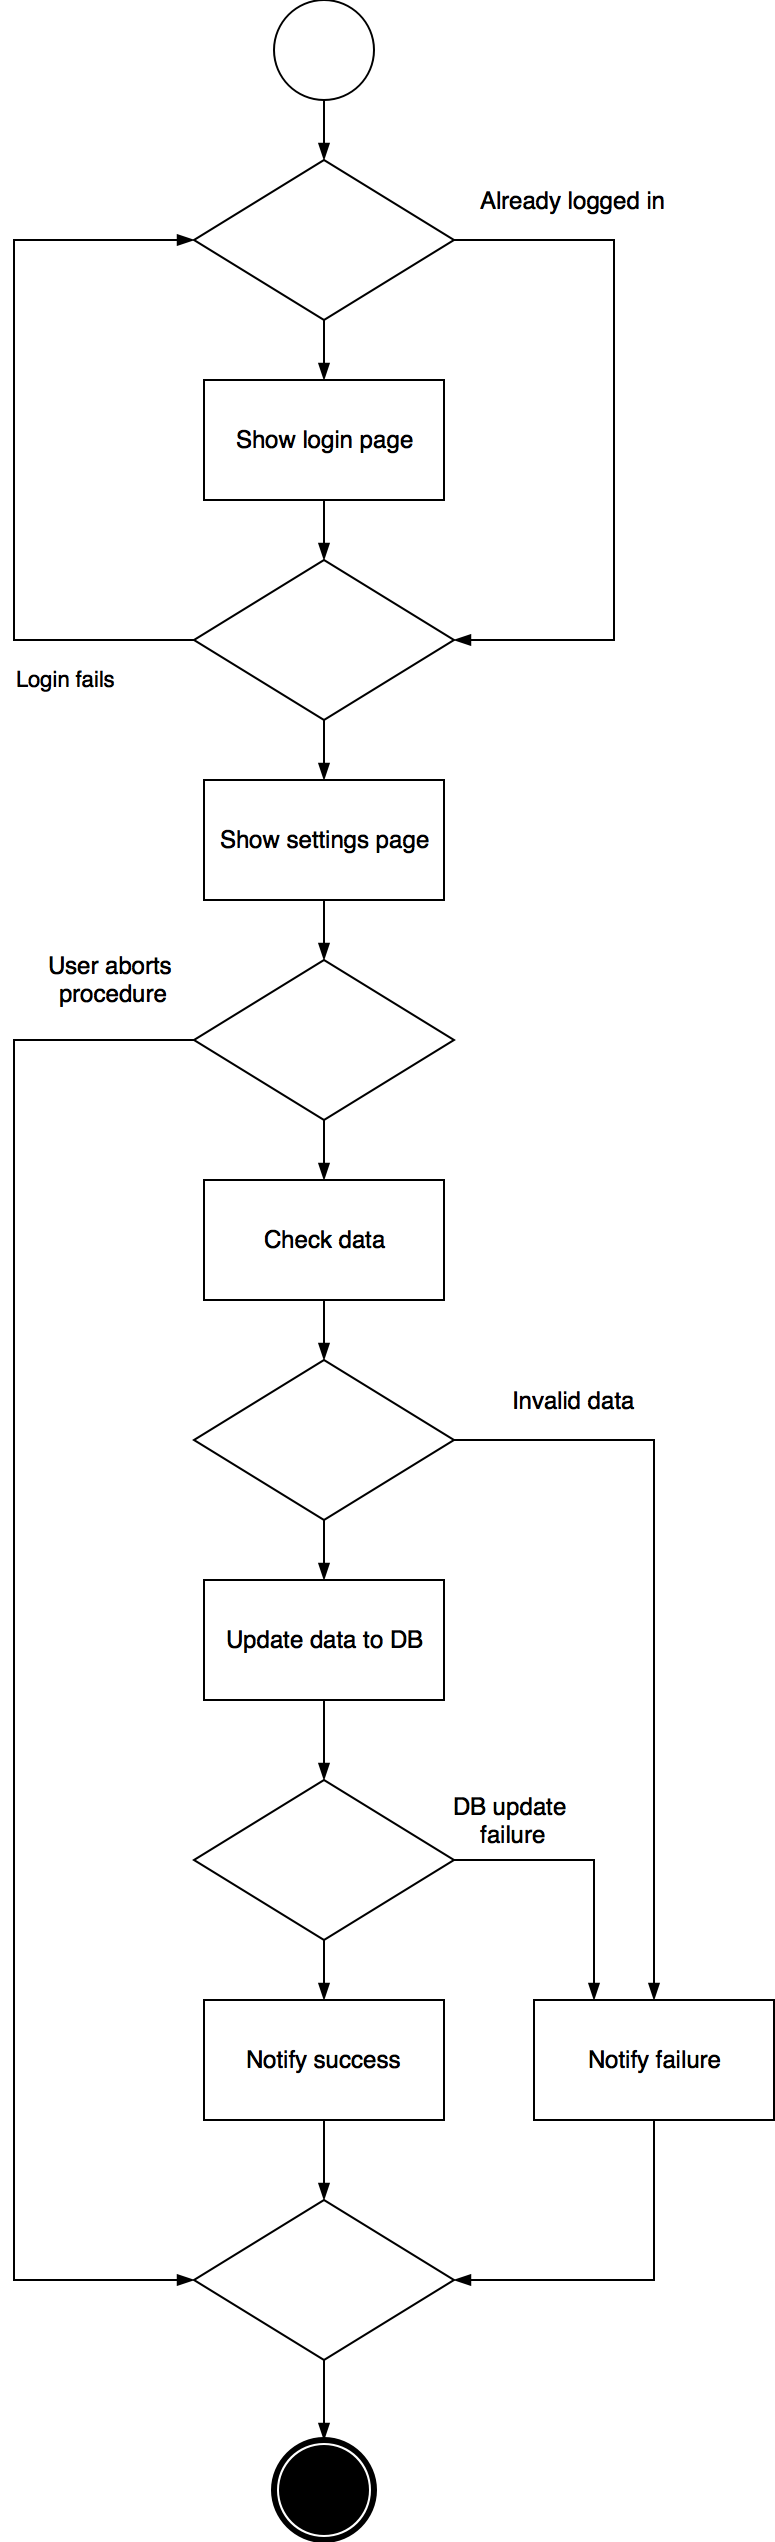
\includegraphics[scale=0.23]{img/diagrams/specify_lunch_timing_ad.png}
		\caption{Activity diagram for Specify lunch timing.}
	\end{figure}

	
	\subsection{Performance requiremens}
	In order to guarantee the best user experience, the following performance requirements must be satisfied by the system:
	\begin{itemize}
		\item The system must be operative 24 hours a day, 7 days a week with an uptime of at least 99\%;
		\item There must not be an upper bound to the number of users registered to the system;
		\item There must not be an upper bound to the number of meetings that each user can insert; 
		\item The system must handle at least 1000 logged users at the same time;
		\item 95\% of the requests must be handled in at least 1 second; \footnotemark[1]
		\item 99\%  of the requests must be handled in at least 3 seconds. \footnotemark[1]
	\end{itemize}
	
	\bigskip
	\noindent
	\footnotemark[1]{ \textit{not taking in count the time spent to communicate with other actors (e.g., Traffic info provider).}}
	
	
	\subsection{Software System Attributes}
	
	
	\subsubsection{Reliability}
	Reliability can be expressed as a percentage on the total operations that succeeds, then we can write the following relation:
	
	\bigskip
	\begin{center}
		\textit{Reliability}  = 100\% - (\textit{probability of Failure} * 100)
	\end{center}

	\bigskip
	The system must have a reliability greater or equal than 99.9\%, that means that failing the operations are less than 0.1\%.

	
	\subsubsection{Availability}
	The system must be up at least 99\% of the time with the exception of ordinary maintenance work.
	
	
	\subsubsection{Security}
	The security attribute depends on the following factors:
	\begin{itemize}
		\item Every communication between application server and client must comply the  HTTPS protocol.
		\item Communication between different servers must be SSL/TLS encrypted.
		\item Sensitive informations (i.e. password) must be properly stored (i.e., key-hashed salted hash).
	\end{itemize}
	
	
	\subsubsection{Mantainability}
	Code and the documentation must match in order to make the code easy to understand for future maintainers.
	
	
	\subsubsection{Portability}
	The back-end application must be written in Java EE7 in order to be able to run on every server that runs JEE7. The web application must support at least the main modern browser (e.g., IE, Firefox, Chrome, Safari). The mobile application must be developed both for IOS and Android.


	\newpage
	\subsubsection{Class Diagram} 

	\begin{figure}[h!]
		\bigskip
		\centering
		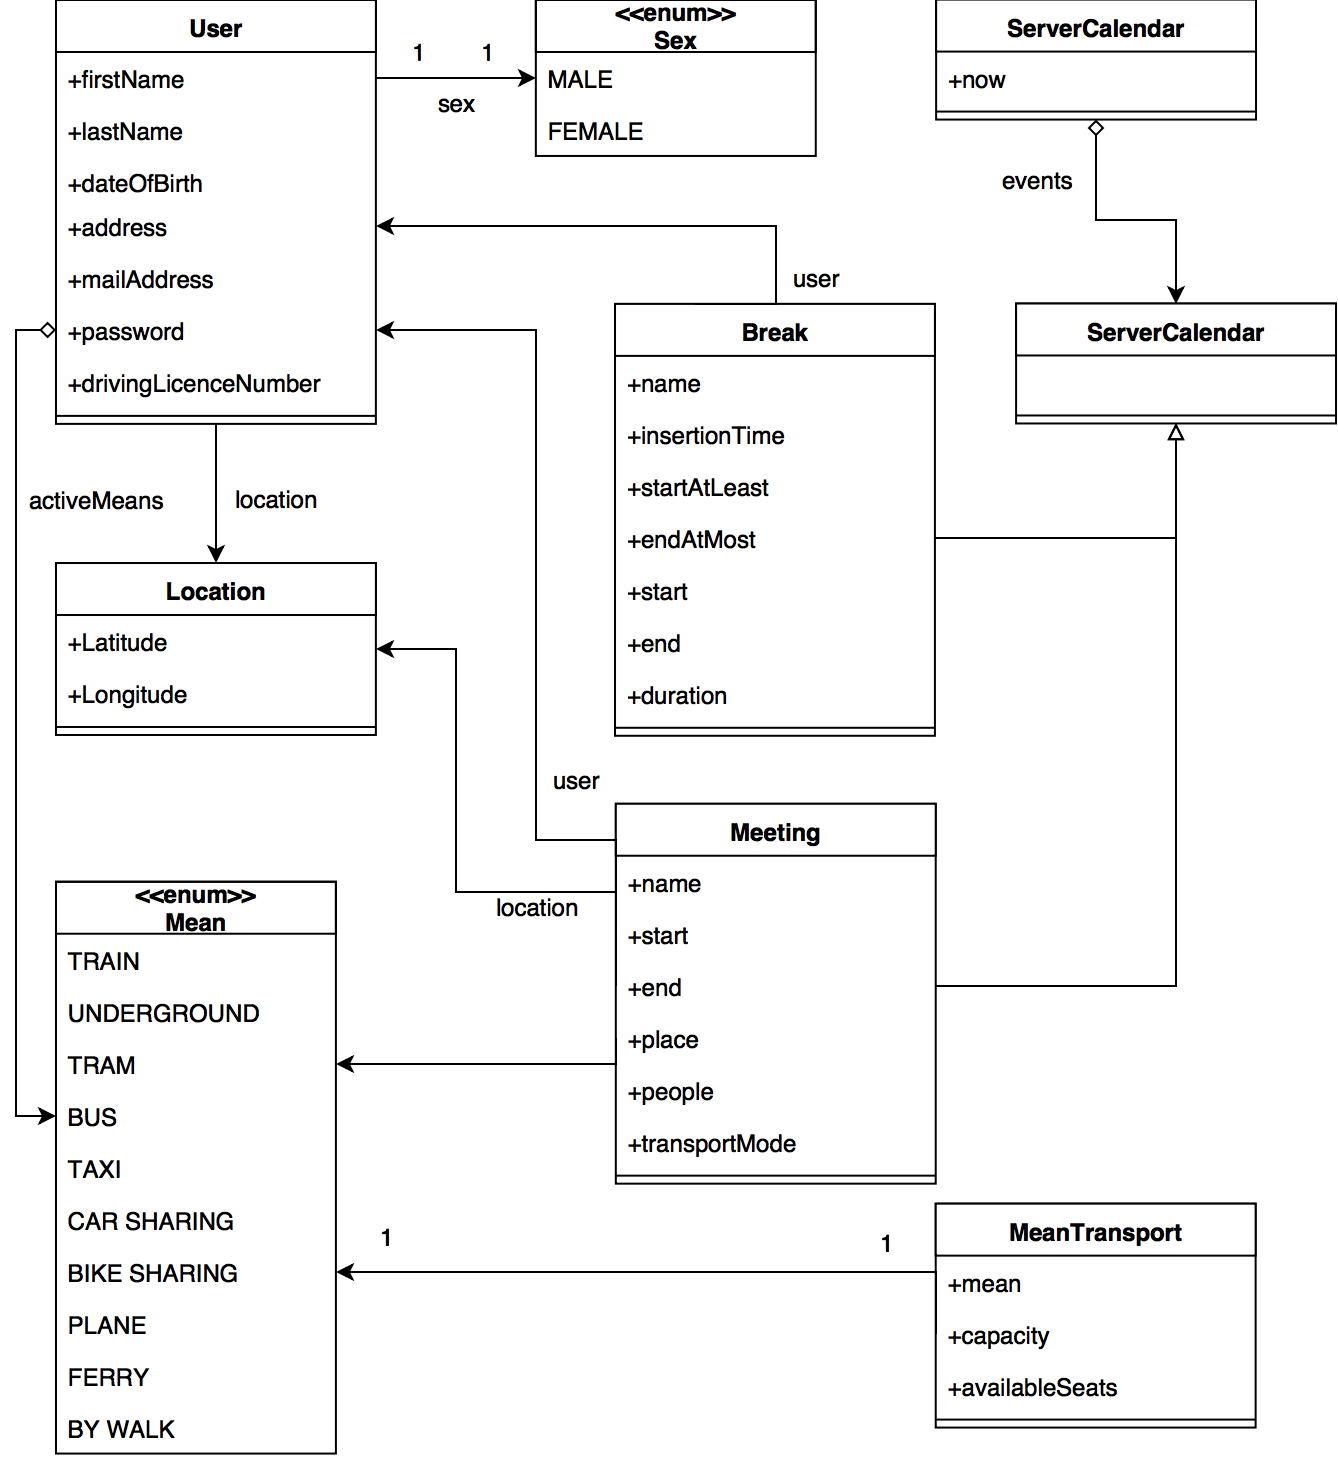
\includegraphics[scale=0.25]{img/diagrams/cd.png}
		\caption{Class Diagram.}
	\end{figure}
	
	
	\section{Formal Analysis Using Alloy}

	\begin{lstlisting}
	
	//SIGNATURES

	one sig ServerCalendar{
		events: set Event,
		now: one Int //current date
	}
	{
		#events >= 0
		now     >= 0
	}

	sig User{
		firstName:            one StringLetter,
		lastName:             one StringLetter,
		dateOfBirth:          one Int,
		sex:                  one Sex,
		mailAddress:          one StringLetter,
		password:             one StringLetter,
		drivingLicenceNumber: lone Int,
		userMeans:            some Mean
	}
	{
		drivingLicenceNumber > 0
	}

	abstract sig Event {}

	sig Meeting extends Event{
	    user:          one User,
		name:          one StringLetter,
		insertionTime: one Int,
		start:         one Int,
		end:           one Int,
		place:         one Location,
		people:        one Int
	}
	{
		insertionTime >= 0
		start         >= 0
		end           >  0
		end           >  start
	}

	//Supposing that duration is an integer attribute
	sig Break extends Event{
	    user:          one User,
		name:          one StringLetter,
		insertionTime: one Int, //date of insertion the break into the calendar
		startAtLeast:  one Int,
		endAtMost:     one Int,
		start:         one Int,
		end:           one Int,
		duration:      one Int
	}
	{
		insertionTime >= 0
		start         <  end
		startAtLeast  <  endAtMost
		start         >= 0
		end           >  0
		startAtLeast  >= 0
		endAtMost     >  0
		duration      >  0
		duration      =  end - start
		start         >= startAtLeast
		end           <= endAtMost
	}

	abstract sig Mean{
		capacity:        one Int,
		available_seats: one Int
	}
	{
		capacity>0
		available_seats >= 0
		available_seats <= capacity
	}

	sig TRAIN       extends Mean {}
	sig UNDERGROUND extends Mean {}
	sig TRAM        extends Mean {}
	sig BUS         extends Mean {}
	sig TAXI        extends Mean {}
	sig CARSHARING  extends Mean {}
	sig BIKESHARING extends Mean {}
	sig PLANE       extends Mean {}
	sig FERRY       extends Mean {}
	sig BYWALK      extends Mean {}

	sig Location{
		latitude:  one Int,
		longitude: one Int
	}
	{    
		latitude  >= -90
		latitude  <= 90
		longitude >= -180
		longitude <= 180
	}

	abstract sig Sex {}
	one sig Male   extends Sex{}
	one sig Female extends Sex{}

	sig StringLetter{}


	// PREDICATES

	pred insertMeeting [s, s': ServerCalendar, m: Meeting] {
		s'.events = s.events + m
		m.insertionTime >= s.now
		m.insertionTime <= s'.now
	}

	pred insertBreak [s, s': ServerCalendar,b: Break] {
		s'.events = s.events + b
		b.insertionTime >= s.now
		b.insertionTime <= s'.now
	}

	pred removeMeeting [s, s': ServerCalendar, m: Meeting] {
		s'.events = s.events - m
	}

	pred removeBreak [s, s': ServerCalendar, b: Break] {
		s'.events= s.events - b
	}

	pred overlapsMM[m1, m2: Meeting] {
	    m1.user = m2.user implies
		((m1.start < m2.start and m1.end  >m2.start) or
		(m1.start >= m2.start and m1.start < m2.end))
	}

	pred overlapsMB[m: Meeting, b: Break] {
	    m.user = b.user implies
		((m.start < b.start and m.end > b.start) or
		(m.start >= b.start and m.start < b.end))
	}

	pred overlapsBB[b1, b2: Break] {
	    b1.user = b2.user implies
		((b1.start < b2.start and b1.end  >b2.start) or
		(b1.start >= b2.start and b1.start < b2.end))
	}


	//FACTS

	//No two distinct overlapping position
	fact NoPositionOverlapping{
		no disj pos1, pos2: Location|
		(pos1.latitude = pos2.latitude and pos1.longitude = pos2.longitude)
	}

	//No two distinct coinciding users
	fact UniqueUser{
		no disj u1, u2: User|
		(u1 != u2 and
		(u1.mailAddress = u2.mailAddress or
		u1.drivingLicenceNumber = u2.drivingLicenceNumber))
	}

	//No two distinct overlapping meeting
	fact UniqueMeeting{
		no disj m1, m2: Meeting|
		(m1 != m2 and
		(m1.user = m2.user or
	    m1.start = m2.start or
		m1.end = m2.end))
	}

	//No two distinct overlapping break
	fact UniqueBreak{
		no disj b1, b2: Break|
		(b1 != b2 and
		(b1.user = b2.user or
	    b1.startAtLeast = b2.startAtLeast or
		b1.endAtMost = b2. endAtMost ))
	}

	//No meeting overlapping meeting
	fact NoMeetingOverlappingMeeting {
		no disj m1, m2:Meeting | overlapsMM[m1, m2]
	}

	//No meeting overlapping break
	fact NoMeetingOverlappingBreak {
		no disj m:Meeting, b: Break | overlapsMB[m, b]
	}

	//No break overlapping break
	fact NoBreakOverlappingBreak {
		no disj b1, b2: Break | overlapsBB[b1, b2]
	}

	//time for break
	fact TimeBreak{
		all b:Break | ((b.endAtMost - b.startAtLeast) >= b.duration)
	}

	//date of meeting is after date of insertion
	fact meetingMustBeInFuture{
		all m: Meeting | (m.insertionTime <= m.start)
	}

	//date of meeting is after date of insertion
	fact breakMustBeInFuture{
		all b: Break | (b.insertionTime <= b.start)
	}

	//Server Calendar contains all breaks
	fact containAllMeetings {
		all m: Meeting, c: ServerCalendar | (m in c.events)
	}

	//Server Calendar contains all breaks
	fact containAllBreaks {
		all b: Break, c: ServerCalendar | (b in c.events)
	}

	//duration break
	fact breakDuration{
		all b: Break | (b.end - b.start = b.duration)
	}

	//The number of people must be lower than the capacity of mean
	fact ContainPeople{
		all m: Meeting, t: Mean | (m.people <= t.capacity)
	}

	//The number of people must be lower than the available seats
	fact AvailablePeople{
		all m:Meeting, t: Mean| (m.people <= t.available_seats)
	}


	//ASSERTIONS

	//No overlps
	assert noOverlapping {
	  no disj m1, m2: Meeting | overlapsMM[m1, m2]
	  no disj m: Meeting, b: Break | overlapsMB[m, b]
	  no disj b1, b2: Break | overlapsBB[b1, b2]
	}
	//Available seats imply higher capacity of the means of transport
	assert available {
		all m:Meeting, t: Mean | ((m.people <= t.available_seats) implies (m.people <= t.capacity))
	}

	//Duration of break is equal to difference between end and start time
	assert breakBuration{
		all b: Break | (b.duration = (b.end - b.start))
	}

	pred show() {}

	run show for 15

	\end{lstlisting}


	\newpage
	Here is the execution of checks on the assertions:

	\bigskip
	\begin{lstlisting}{numbers=none}
	Executing "Check noOverlapping for 25"
	   Solver=sat4j Bitwidth=4 MaxSeq=7 SkolemDepth=1 Symmetry=20
	   408265 vars. 13116 primary vars. 1170897 clauses. 9215ms.
	   No counterexample found. Assertion may be valid. 146ms.

	Executing "Check available for 25"
	   Solver=sat4j Bitwidth=4 MaxSeq=7 SkolemDepth=1 Symmetry=20
	   408796 vars. 13166 primary vars. 921430 clauses. 4645ms.
	   No counterexample found. Assertion may be valid. 1133ms.

	Executing "Check reakBuration for 25"
	   Solver=sat4j Bitwidth=4 MaxSeq=7 SkolemDepth=1 Symmetry=20
	   408224 vars. 13141 primary vars. 920158 clauses. 3455ms.
	   No counterexample found. Assertion may be valid. 387ms.
	\end{lstlisting}

	\begin{figure}[h!]
		\bigskip
		\centering
		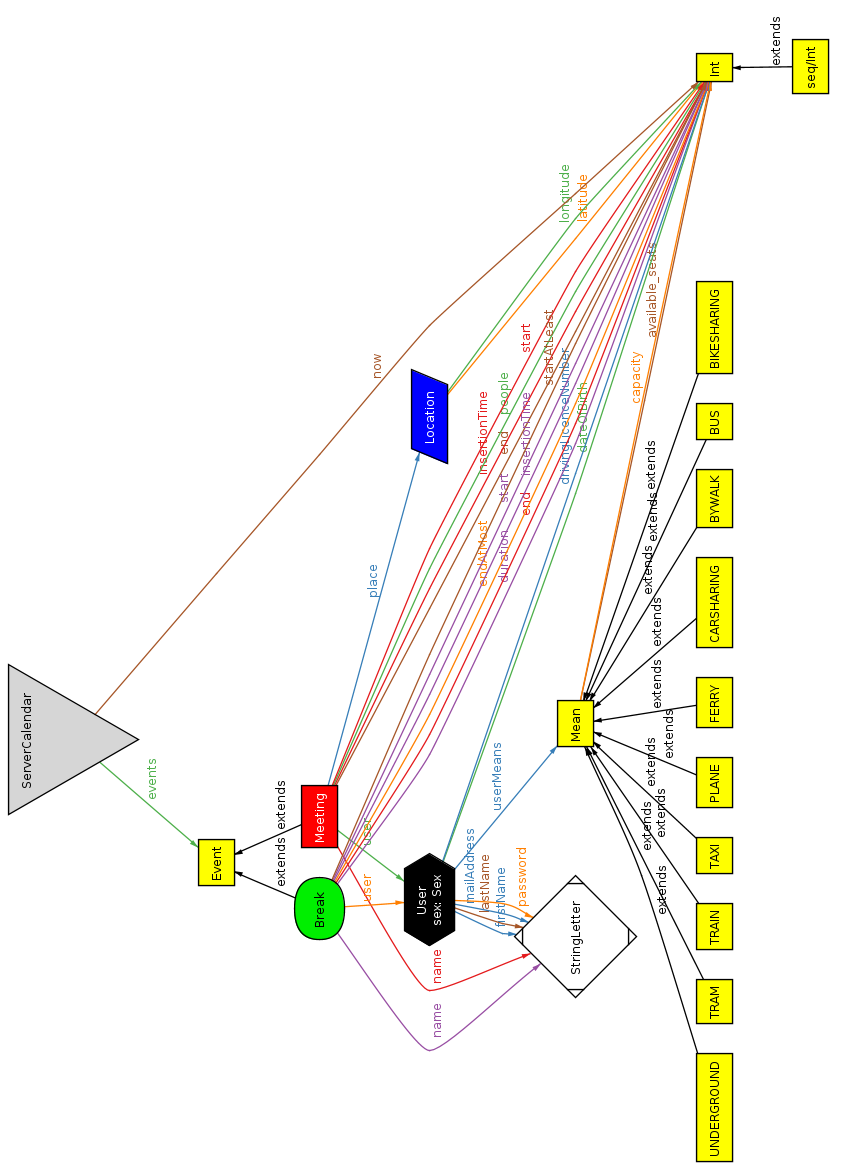
\includegraphics[scale=0.5]{img/diagrams/mm.png}
		\caption{Metamodel.}
	\end{figure}
	\begin{figure}[h!]
		\bigskip
		\centering
		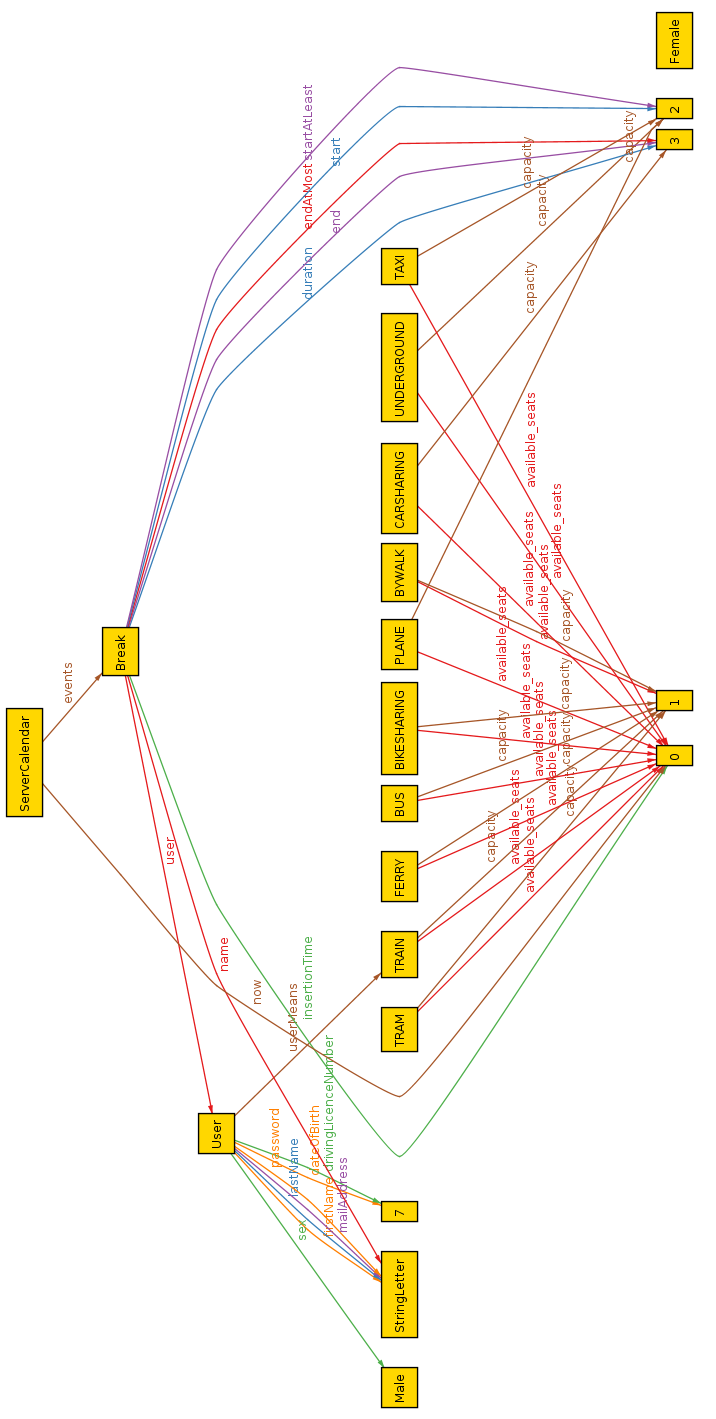
\includegraphics[scale=0.4]{img/diagrams/i.png}
		\caption{An Alloy instance.}
	\end{figure}
	\newpage
	\appendix
	\section{Appendix}

	\subsection{Software and tools used}
	The software and tools used during the drawing of this document are:
	\begin{description}
		\item[LaTex:] used to build this document.
		\item[Google Drive / Google Documents:] used to always update and share the documents.
		\item[draw.io:] used to draw diagrams (https://www.draw.io).
		\item[Marvel:] used to build the mockups (https://marvelapp.com).
		\item[GitHub:] used as version control and to keep it shared between group members and teachers (https://www.github.com).
		\item[Alloy Analyzer:] used to analyze specifications and requirements.
	\end{description}


	\subsection{Hours of work}
	Most of the work on this document was made in the presence of both members of the group. The approximate number of hours worked by each member of the group is as follow (including hours spent in group work):

	\bigskip
	Davide Rossetto: about 40 hours
	
	Alessandro Tatti: about 40 hours


	\section{Bibliography}

	[1] AA 2017/2018 Software Engineering 2 - Project goal, schedule and rules
	
	\noindent
	\bigskip
	[2] Jackson, Zave - The World and the Machine

\end{document}
